\documentclass[aspectratio=169,10pt]{beamer}
\usepackage[utf8]{inputenc}
\usepackage[english]{babel}
\usepackage{graphicx}
\usepackage{listings}
\usepackage{xcolor}
\usepackage{tikz}
\usepackage{forest}
\usepackage{amsmath}
\usepackage{amssymb}
\usepackage{hyperref}
\usepackage{multicol}
\usepackage{fancyvrb}

\usetikzlibrary{shapes.geometric, arrows, positioning, shadows, calc, backgrounds}

% Tema e colori
\usetheme{Madrid}
\usecolortheme{whale}

% Definizione colori personalizzati
\definecolor{mysqlblue}{RGB}{0,117,143}
\definecolor{phpblue}{RGB}{119,135,179}
\definecolor{codegreen}{RGB}{0,128,0}
\definecolor{codegray}{RGB}{128,128,128}
\definecolor{codepurple}{RGB}{153,0,153}
\definecolor{backcolour}{RGB}{245,245,245}

% Configurazione listings per PHP
\lstdefinestyle{phpstyle}{
    language=PHP,
    backgroundcolor=\color{backcolour},   
    commentstyle=\color{codegreen},
    keywordstyle=\color{blue}\bfseries,
    numberstyle=\tiny\color{codegray},
    stringstyle=\color{codepurple},
    basicstyle=\ttfamily\footnotesize,
    breakatwhitespace=false,         
    breaklines=true,                 
    captionpos=b,                    
    keepspaces=true,                 
    numbers=left,                    
    numbersep=5pt,                  
    showspaces=false,                
    showstringspaces=false,
    showtabs=false,                  
    tabsize=2,
    frame=single,
    rulecolor=\color{mysqlblue}
}

\lstset{style=phpstyle}

% Stile per SQL
\lstdefinestyle{sqlstyle}{
    language=SQL,
    backgroundcolor=\color{backcolour},   
    commentstyle=\color{codegreen},
    keywordstyle=\color{mysqlblue}\bfseries,
    numberstyle=\tiny\color{codegray},
    stringstyle=\color{codepurple},
    basicstyle=\ttfamily\footnotesize,
    breakatwhitespace=false,         
    breaklines=true,                 
    captionpos=b,                    
    keepspaces=true,                 
    numbers=left,                    
    numbersep=5pt,                  
    showspaces=false,                
    showstringspaces=false,
    showtabs=false,                  
    tabsize=2,
    frame=single,
    rulecolor=\color{mysqlblue}
}

% Informazioni del documento
\title{PHP - MySQLi}
\subtitle{Interazione tra PHP e Database MySQL}
\author{Fedeli Massimo}
\institute{IIS E.Fermi - Sacconi - Ceci}
\date{Tutti i diritti riservati}

\begin{document}

% ====================
% SLIDE 1 - Copertina
% ====================
\begin{frame}
\titlepage
\begin{center}

\begin{tikzpicture}[scale=0.6]
    % Logo PHP simbolico
    \fill[phpblue] (0,0) ellipse (1.5cm and 1cm);
    \node[white,font=\Large\bfseries] at (0,0) {PHP};
    % Freccia di connessione
    \draw[->,line width=2pt,mysqlblue] (2,0) -- (4,0);
    % Logo MySQL simbolico
    \fill[mysqlblue] (5.5,0) ellipse (1.5cm and 1cm);
    \node[white,font=\Large\bfseries] at (5.5,0) {MySQL};
\end{tikzpicture}
\end{center}
\end{frame}

% ====================
% SLIDE 2 - Indice
% ====================
\begin{frame}{Indice}
\tableofcontents
\end{frame}

% ====================
% SEZIONE 1: MYSQL
% ====================
\section{Il DBMS MySQL}

% ====================
% SLIDE 3
% ====================
\begin{frame}{Il DBMS MySQL}
\begin{columns}
\begin{column}{0.6\textwidth}
\textbf{MySQL} è un DBMS Server con le seguenti caratteristiche:
\begin{itemize}
    \item Basato su SQL
    \item Multipiattaforma
    \item Relazionale
    \item Licenza open source
\end{itemize}

\vspace{0.5cm}
\textbf{Avvio del servizio:}
\begin{enumerate}
    \item Aprire il pannello XAMPP
    \item Fare clic su "Start" accanto a MySQL
    \item Accedere a phpMyAdmin tramite "Admin"
\end{enumerate}
\end{column}

\begin{column}{0.4\textwidth}

\begin{tikzpicture}[scale=0.8]
    % Server rappresentazione
    \draw[fill=mysqlblue!20,draw=mysqlblue,line width=1.5pt] (0,0) rectangle (3,4);
    \node[mysqlblue,font=\Large\bfseries] at (1.5,3.3) {MySQL};
    \node[mysqlblue,font=\Large\bfseries] at (1.5,2.8) {Server};
    
    % Dischi del database
    \foreach \y in {2.2,1.7,1.2,0.7}
        \draw[fill=mysqlblue!40,draw=mysqlblue] (0.5,\y) rectangle (2.5,\y+0.3);
    
    % Icona di accesso
    \draw[fill=green!30,draw=green!60!black,line width=1pt] (1,0.2) circle (0.3);
    \node[font=\tiny] at (1.5,0.2) {START};
\end{tikzpicture}
\end{column}
\end{columns}
\end{frame}

% ====================
% SLIDE 4
% ====================
\begin{frame}{Pannello di controllo XAMPP}
\begin{center}
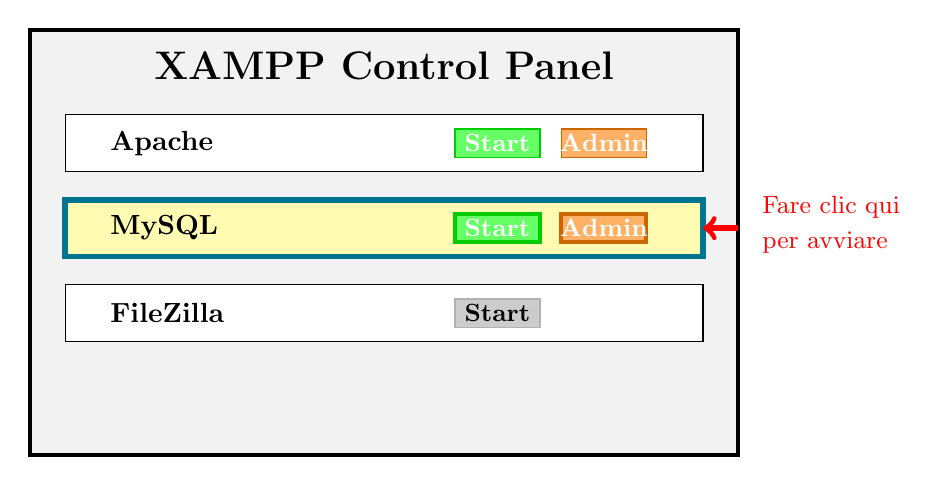
\begin{tikzpicture}[scale=0.9]
    % Finestra XAMPP
    \draw[fill=gray!10,draw=black,line width=1.5pt] (0,0) rectangle (10,6);
    \node[font=\Large\bfseries] at (5,5.5) {XAMPP Control Panel};
    
    % Apache
    \draw[fill=white,draw=black] (0.5,4) rectangle (9.5,4.8);
    \node[anchor=west] at (1,4.4) {\textbf{Apache}};
    \draw[fill=green!60,draw=green!80!black] (6,4.2) rectangle (7.2,4.6);
    \node[white,font=\small\bfseries] at (6.6,4.4) {Start};
    \draw[fill=orange!60,draw=orange!80!black] (7.5,4.2) rectangle (8.7,4.6);
    \node[white,font=\small\bfseries] at (8.1,4.4) {Admin};
    
    % MySQL - evidenziato
    \draw[fill=yellow!30,draw=mysqlblue,line width=2pt] (0.5,2.8) rectangle (9.5,3.6);
    \node[anchor=west,font=\bfseries] at (1,3.2) {MySQL};
    \draw[fill=green!60,draw=green!80!black,line width=1.5pt] (6,3) rectangle (7.2,3.4);
    \node[white,font=\small\bfseries] at (6.6,3.2) {Start};
    \draw[fill=orange!60,draw=orange!80!black,line width=1.5pt] (7.5,3) rectangle (8.7,3.4);
    \node[white,font=\small\bfseries] at (8.1,3.2) {Admin};
    
    % FileZilla
    \draw[fill=white,draw=black] (0.5,1.6) rectangle (9.5,2.4);
    \node[anchor=west] at (1,2) {\textbf{FileZilla}};
    \draw[fill=gray!40,draw=gray!60] (6,1.8) rectangle (7.2,2.2);
    \node[font=\small\bfseries] at (6.6,2) {Start};
    
    % Annotazione
    \draw[->,red,line width=2pt] (10,3.2) -- (9.5,3.2);
    \node[red,anchor=west,font=\small] at (10.2,3.5) {Fare clic qui};
    \node[red,anchor=west,font=\small] at (10.2,3.0) {per avviare};
\end{tikzpicture}
\end{center}
\end{frame}

% ====================
% SLIDE 5
% ====================
\begin{frame}{phpMyAdmin - Ambiente di Amministrazione}
\begin{itemize}
    \item \textbf{phpMyAdmin} è l'ambiente di amministrazione grafico per MySQL
    \item Permette di gestire database e tabelle tramite interfaccia GUI
    \item Accessibile tramite browser web
\end{itemize}

\vspace{0.5cm}
\begin{center}
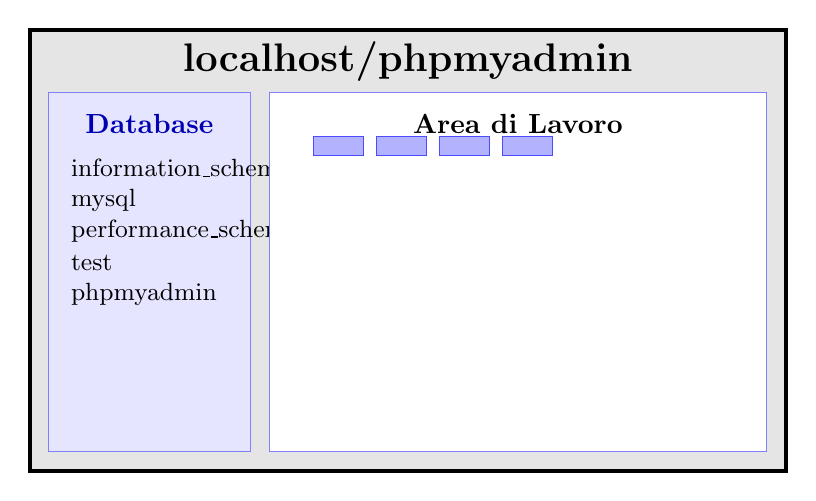
\begin{tikzpicture}[scale=0.8]
    % Browser
    \draw[fill=gray!20,draw=black,line width=1.5pt] (0,0) rectangle (12,7);
    \node[font=\Large\bfseries] at (6,6.5) {localhost/phpmyadmin};
    
    % Colonna sinistra - Database
    \draw[fill=blue!10,draw=blue!50] (0.3,0.3) rectangle (3.5,6);
    \node[font=\bfseries,blue!70!black] at (1.9,5.5) {Database};
    \foreach \db/\y in {information\_schema/4.8, mysql/4.3, performance\_schema/3.8, test/3.3, phpmyadmin/2.8}
        \node[anchor=west,font=\small] at (0.5,\y) {\db};
    
    % Area principale
    \draw[fill=white,draw=blue!50] (3.8,0.3) rectangle (11.7,6);
    \node[font=\bfseries] at (7.75,5.5) {Area di Lavoro};
    
    % Tabs
    \foreach \tab/\x in {Struttura/4.5, SQL/5.5, Ricerca/6.5, Inserisci/7.5}
        \draw[fill=blue!30,draw=blue!70] (\x,5) rectangle (\x+0.8,5.3);
\end{tikzpicture}
\end{center}
\end{frame}

% ====================
% SLIDE 6
% ====================
\begin{frame}{Selezione Database in phpMyAdmin}
\begin{columns}
\begin{column}{0.5\textwidth}
\textbf{Operazioni disponibili:}
\begin{enumerate}
    \item Selezionare un database dalla colonna sinistra
    \item Espandere il simbolo "+" per vedere le tabelle
    \item Fare clic sul nome per accedere alle funzioni
\end{enumerate}

\vspace{0.3cm}
Esempio: database \texttt{test}
\end{column}

\begin{column}{0.5\textwidth}
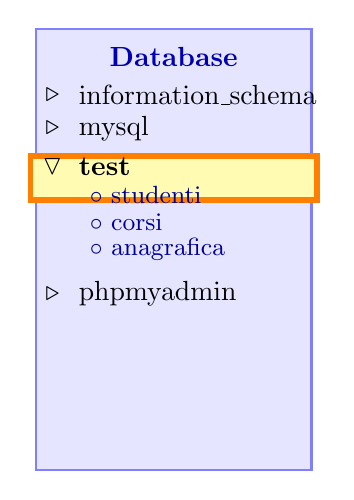
\begin{tikzpicture}[scale=0.7]
    \draw[fill=blue!10,draw=blue!50,line width=1pt] (0,0) rectangle (5,8);
    \node[font=\bfseries,blue!70!black] at (2.5,7.5) {Database};
    
    % Database collassato
    \node at (0.3,6.8) {$\triangleright$};
    \node[anchor=west] at (0.6,6.8) {information\_schema};
    
    \node at (0.3,6.2) {$\triangleright$};
    \node[anchor=west] at (0.6,6.2) {mysql};
    
    % Database test espanso - evidenziato
    \draw[fill=yellow!30,draw=orange,line width=2pt] (-0.1,4.9) rectangle (5.1,5.7);
    \node at (0.3,5.5) {$\triangledown$};
    \node[anchor=west,font=\bfseries] at (0.6,5.5) {test};
    
    % Tabelle del database test
    \node[anchor=west,font=\small,blue!60!black] at (0.8,5) {$\circ$ studenti};
    \node[anchor=west,font=\small,blue!60!black] at (0.8,4.5) {$\circ$ corsi};
    \node[anchor=west,font=\small,blue!60!black] at (0.8,4) {$\circ$ anagrafica};
    
    \node at (0.3,3.2) {$\triangleright$};
    \node[anchor=west] at (0.6,3.2) {phpmyadmin};
\end{tikzpicture}
\end{column}
\end{columns}
\end{frame}

% ====================
% SEZIONE 2: MYSQLI
% ====================
\section{L'interfaccia MySQLi}

% ====================
% SLIDE 7
% ====================
\begin{frame}{La Classe MySQLi}
\begin{block}{Caratteristiche Principali}
PHP dispone della classe \texttt{mysqli} per l'interazione con il DBMS MySQL
\end{block}

\vspace{0.5cm}
\begin{columns}
\begin{column}{0.5\textwidth}
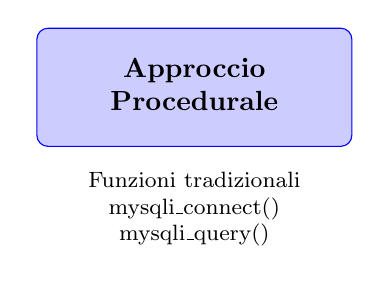
\begin{tikzpicture}[scale=0.9]
    % Approccio Procedurale
    \node[rectangle,draw=blue,fill=blue!20,minimum width=4cm,minimum height=1.5cm,rounded corners] (proc) at (0,0) {
        \begin{tabular}{c}
        \textbf{Approccio} \\
        \textbf{Procedurale}
        \end{tabular}
    };
    \node[below=0.2cm of proc,font=\footnotesize,text width=4cm,align=center] {
        Funzioni tradizionali \\
        mysqli\_connect() \\
        mysqli\_query()
    };
\end{tikzpicture}
\end{column}

\begin{column}{0.5\textwidth}
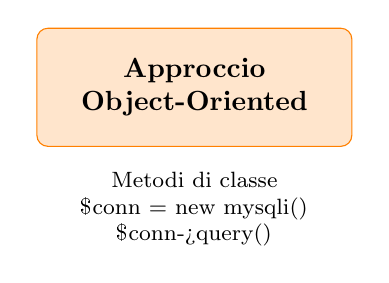
\begin{tikzpicture}[scale=0.9]
    % Approccio OOP
    \node[rectangle,draw=orange,fill=orange!20,minimum width=4cm,minimum height=1.5cm,rounded corners] (oop) at (0,0) {
        \begin{tabular}{c}
        \textbf{Approccio} \\
        \textbf{Object-Oriented}
        \end{tabular}
    };
    \node[below=0.2cm of oop,font=\footnotesize,text width=4cm,align=center] {
        Metodi di classe \\
        \$conn = new mysqli() \\
        \$conn->query()
    };
\end{tikzpicture}
\end{column}
\end{columns}

\vspace{0.5cm}
\begin{center}
\textit{I due approcci possono essere utilizzati nello stesso script!}
\end{center}
\end{frame}

% ====================
% SLIDE 8
% ====================
\begin{frame}{Interfaccia MySQLi - Vantaggi}
\begin{center}
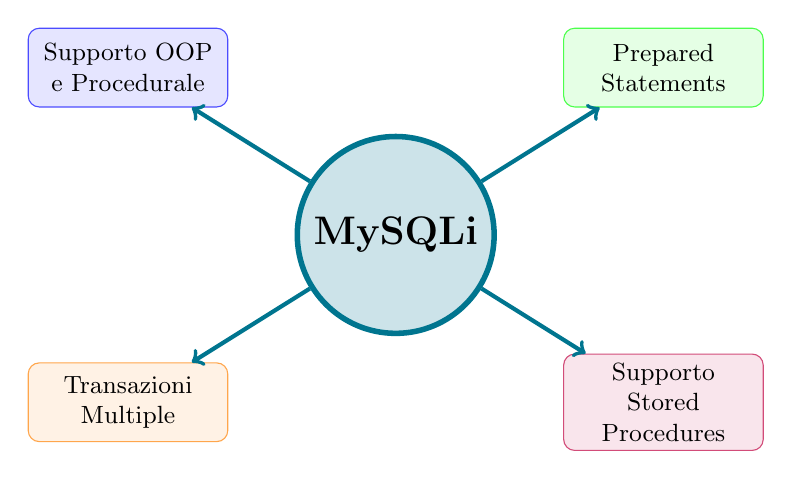
\begin{tikzpicture}[scale=0.85]
    % Nodo centrale
    \node[circle,draw=mysqlblue,fill=mysqlblue!20,minimum size=2.5cm,line width=2pt,font=\Large\bfseries] (center) at (0,0) {MySQLi};
    
    % Vantaggi disposti a raggiera
    \node[rectangle,draw=blue!70,fill=blue!10,minimum width=2.5cm,minimum height=1cm,rounded corners,font=\small,text width=2.3cm,align=center] (v1) at (-4,2.5) {Supporto OOP e Procedurale};
    
    \node[rectangle,draw=green!70,fill=green!10,minimum width=2.5cm,minimum height=1cm,rounded corners,font=\small,text width=2.3cm,align=center] (v2) at (4,2.5) {Prepared Statements};
    
    \node[rectangle,draw=orange!70,fill=orange!10,minimum width=2.5cm,minimum height=1cm,rounded corners,font=\small,text width=2.3cm,align=center] (v3) at (-4,-2.5) {Transazioni Multiple};
    
    \node[rectangle,draw=purple!70,fill=purple!10,minimum width=2.5cm,minimum height=1cm,rounded corners,font=\small,text width=2.3cm,align=center] (v4) at (4,-2.5) {Supporto Stored Procedures};
    
    % Connessioni
    \draw[->,line width=1.5pt,mysqlblue] (center) -- (v1);
    \draw[->,line width=1.5pt,mysqlblue] (center) -- (v2);
    \draw[->,line width=1.5pt,mysqlblue] (center) -- (v3);
    \draw[->,line width=1.5pt,mysqlblue] (center) -- (v4);
\end{tikzpicture}
\end{center}
\end{frame}

% ====================
% SEZIONE 3: CONNESSIONE
% ====================
\section{Connessione al Database}

% ====================
% SLIDE 9
% ====================
\begin{frame}[fragile]{Connessione al Database - Sintassi}
\begin{block}{Sintassi Object-Oriented}
\begin{lstlisting}[style=phpstyle]
$conn = new mysqli($nomeHost, $username, $password, $dbname);
\end{lstlisting}
\end{block}

\vspace{0.3cm}
\textbf{Parametri:}
\begin{description}
    \item[\$nomeHost] Macchina che esegue il DBMS (es. "localhost")
    \item[\$username] Utente per l'accesso al database (es. "root")
    \item[\$password] Password associata all'utente
    \item[\$dbname] Nome del database da utilizzare
\end{description}

\vspace{0.3cm}
\begin{alertblock}{Importante}
La variabile \texttt{\$conn} è l'oggetto che rappresenta la connessione al database
\end{alertblock}
\end{frame}

% ====================
% SLIDE 10
% ====================
\begin{frame}[fragile]{Esempio di Connessione}
\begin{lstlisting}[style=phpstyle]
<?php
// Parametri di connessione
$servername = "localhost";
$username = "root";
$password = "";
$dbname = "test";

// Creazione connessione
$conn = new mysqli($servername, $username, $password, $dbname);

// Verifica connessione
if ($conn->connect_error) {
    die("Connessione fallita: " . $conn->connect_error);
}
echo "Connessione riuscita";
?>
\end{lstlisting}
\end{frame}

% ====================
% SLIDE 11
% ====================
\begin{frame}{Valori Restituiti - Stile OOP}
\begin{center}
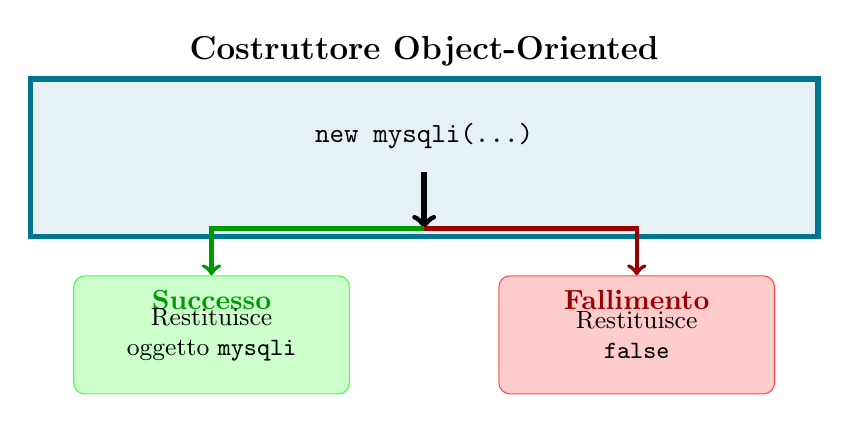
\begin{tikzpicture}[scale=0.9]
    % Box principale
    \node[rectangle,draw=mysqlblue,fill=mysqlblue!10,minimum width=10cm,minimum height=2cm,line width=2pt] (main) at (0,0) {};
    \node[above] at (main.north) {\large\textbf{Costruttore Object-Oriented}};
    
    % Freccia decisione
    \node at (0,0.3) {\texttt{new mysqli(...)}};
    \draw[->,line width=2pt] (0,-0.2) -- (0,-1);
    
    % Successo
    \node[rectangle,draw=green!70,fill=green!20,minimum width=3.5cm,minimum height=1.5cm,rounded corners] (success) at (-3,-2.5) {};
    \node[font=\bfseries,green!60!black] at (success.north) [below=2pt] {Successo};
    \node[font=\small,text width=3cm,align=center] at (success.center) {Restituisce \\ oggetto \texttt{mysqli}};
    
    % Fallimento
    \node[rectangle,draw=red!70,fill=red!20,minimum width=3.5cm,minimum height=1.5cm,rounded corners] (fail) at (3,-2.5) {};
    \node[font=\bfseries,red!60!black] at (fail.north) [below=2pt] {Fallimento};
    \node[font=\small,text width=3cm,align=center] at (fail.center) {Restituisce \\ \texttt{false}};
    
    % Connessioni
    \draw[->,line width=1.5pt,green!60!black] (0,-1) -| (success);
    \draw[->,line width=1.5pt,red!60!black] (0,-1) -| (fail);
\end{tikzpicture}
\end{center}
\end{frame}

% ====================
% SLIDE 12
% ====================
\begin{frame}{Valori Restituiti - Stile Procedurale}
\begin{center}
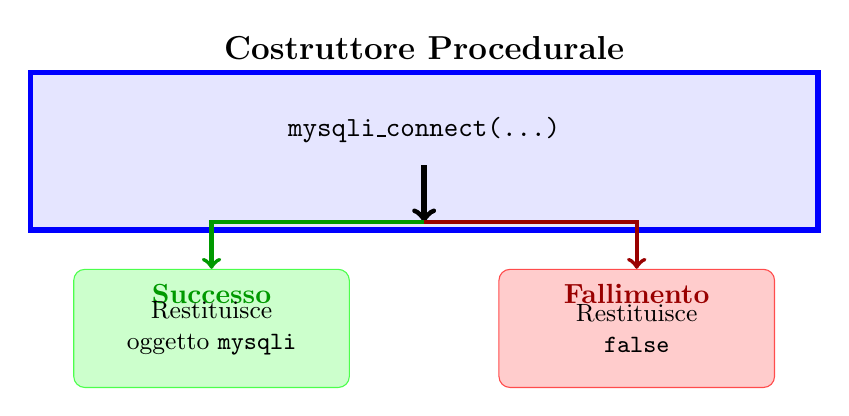
\begin{tikzpicture}[scale=0.9]
    % Box principale
    \node[rectangle,draw=blue,fill=blue!10,minimum width=10cm,minimum height=2cm,line width=2pt] (main) at (0,0) {};
    \node[above] at (main.north) {\large\textbf{Costruttore Procedurale}};
    
    % Freccia decisione
    \node at (0,0.3) {\texttt{mysqli\_connect(...)}};
    \draw[->,line width=2pt] (0,-0.2) -- (0,-1);
    
    % Successo
    \node[rectangle,draw=green!70,fill=green!20,minimum width=3.5cm,minimum height=1.5cm,rounded corners] (success) at (-3,-2.5) {};
    \node[font=\bfseries,green!60!black] at (success.north) [below=2pt] {Successo};
    \node[font=\small,text width=3cm,align=center] at (success.center) {Restituisce \\ oggetto \texttt{mysqli}};
    
    % Fallimento
    \node[rectangle,draw=red!70,fill=red!20,minimum width=3.5cm,minimum height=1.5cm,rounded corners] (fail) at (3,-2.5) {};
    \node[font=\bfseries,red!60!black] at (fail.north) [below=2pt] {Fallimento};
    \node[font=\small,text width=3cm,align=center] at (fail.center) {Restituisce \\ \texttt{false}};
    
    % Connessioni
    \draw[->,line width=1.5pt,green!60!black] (0,-1) -| (success);
    \draw[->,line width=1.5pt,red!60!black] (0,-1) -| (fail);
\end{tikzpicture}
\end{center}
\end{frame}

% ====================
% SLIDE 13
% ====================
\begin{frame}[fragile]{Il Metodo connect\_errno}
\begin{block}{Descrizione}
Il metodo \texttt{connect\_errno()} verifica se la connessione è avvenuta regolarmente
\end{block}

\vspace{0.3cm}
\textbf{Valore di ritorno:}
\begin{itemize}
    \item \texttt{0} $\rightarrow$ Connessione riuscita
    \item \texttt{Numero diverso da 0} $\rightarrow$ Codice di errore
\end{itemize}

\vspace{0.3cm}
\begin{lstlisting}[style=phpstyle]
if ($conn->connect_errno) {
    echo "Errore connessione: " . $conn->connect_errno;
    exit();
}
\end{lstlisting}

\vspace{0.3cm}
\begin{center}
\small\url{https://www.w3schools.com/php/func_mysqli_connect_errno.asp}
\end{center}
\end{frame}

% ====================
% SLIDE 14
% ====================
\begin{frame}[fragile]{Gestione Errori di Connessione}
\begin{columns}
\begin{column}{0.5\textwidth}
\textbf{Metodi per gestire gli errori:}
\begin{itemize}
    \item \texttt{connect\_errno}: codice errore
    \item \texttt{connect\_error}: descrizione errore
\end{itemize}
\end{column}

\begin{column}{0.5\textwidth}
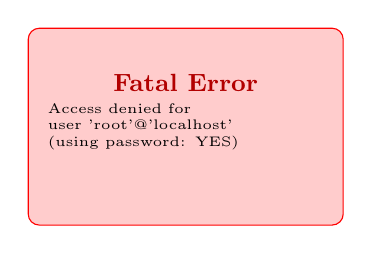
\begin{tikzpicture}[scale=0.7]
    \node[rectangle,draw=red,fill=red!20,minimum width=4cm,minimum height=2.5cm,rounded corners] (error) at (0,0) {};
    \node[font=\bfseries\small,red!70!black] at (0,0.8) {Fatal Error};
    \node[font=\tiny,text width=3.5cm,align=left] at (0,0) {
        Access denied for \\
        user 'root'@'localhost' \\
        (using password: YES)
    };
\end{tikzpicture}
\end{column}
\end{columns}

\vspace{0.3cm}
\begin{lstlisting}[style=phpstyle]
if ($conn->connect_error) {
    die("Connessione fallita: " . $conn->connect_error);
}
\end{lstlisting}

\begin{center}
\small\url{https://www.w3schools.com/php/func_mysqli_connect_error.asp}
\end{center}
\end{frame}

% ====================
% SLIDE 15
% ====================
\begin{frame}[fragile]{Chiusura della Connessione}
\begin{alertblock}{Importante!}
È fondamentale chiudere la connessione al termine dello script per:
\begin{itemize}
    \item Liberare risorse del server
    \item Evitare sovraccarico del Web server
    \item Prevenire problemi di sicurezza
\end{itemize}
\end{alertblock}

\vspace{0.5cm}
\begin{lstlisting}[style=phpstyle]
// Chiusura della connessione
$conn->close();
\end{lstlisting}

\vspace{0.3cm}
\begin{center}
\small\url{https://www.php.net/manual/en/mysqli.close.php}
\end{center}
\end{frame}

% ====================
% SLIDE 16
% ====================
\begin{frame}{Note sulla Chiusura - Documentazione Ufficiale}
\begin{block}{Dalla documentazione PHP}
\textit{``Open non-persistent MySQL connections and result sets are automatically closed when their objects are destroyed. Explicitly closing open connections and freeing result sets is optional.''}
\end{block}

\vspace{0.5cm}
\begin{exampleblock}{Best Practice}
\textit{``However, it's a good idea to close the connection as soon as the script finishes performing all of its database operations, if it still has a lot of processing to do after getting the results.''}
\end{exampleblock}

\vspace{0.3cm}
\begin{center}
\small\url{https://www.php.net/manual/en/mysqli.close.php}
\end{center}
\end{frame}

% ====================
% SEZIONE 4: QUERY
% ====================
\section{Esecuzione Query}

% ====================
% SLIDE 17
% ====================
\begin{frame}[fragile]{Il Metodo query()}
\begin{block}{Descrizione}
Il metodo \texttt{query()} invia una query SQL al database aperto
\end{block}

\vspace{0.3cm}
\textbf{Sintassi:}
\begin{lstlisting}[style=phpstyle]
$result = $conn->query($sql);
\end{lstlisting}

\vspace{0.3cm}
\textbf{Esempio:}
\begin{lstlisting}[style=phpstyle]
$sql = "SELECT * FROM Anagrafica WHERE Cognome LIKE 'Ros%'";
$ris = $conn->query($sql);
\end{lstlisting}

\vspace{0.3cm}
\begin{center}
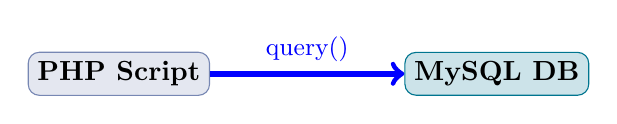
\begin{tikzpicture}[scale=0.8]
    \node[rectangle,draw=phpblue,fill=phpblue!20,rounded corners] (php) at (0,0) {\textbf{PHP Script}};
    \node[rectangle,draw=mysqlblue,fill=mysqlblue!20,rounded corners] (mysql) at (6,0) {\textbf{MySQL DB}};
    \draw[->,line width=2pt,blue] (php) -- node[above,font=\small] {query()} (mysql);
\end{tikzpicture}
\end{center}
\end{frame}

% ====================
% SLIDE 18
% ====================
\begin{frame}{Metodo query() - Parametri}
\begin{block}{Parametri in Ingresso}
\begin{description}
    \item[\$query] (string) La stringa contenente la query SQL da eseguire
\end{description}
\end{block}

\vspace{0.5cm}
\textbf{Tipologie di query supportate:}
\begin{center}
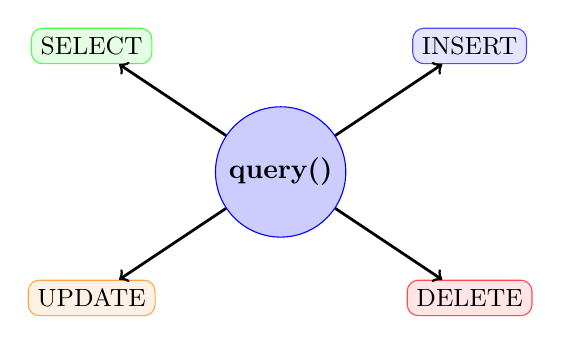
\begin{tikzpicture}[scale=0.8]
    % Nodo centrale
    \node[circle,draw=blue,fill=blue!20,minimum size=1.5cm,font=\bfseries] (center) at (0,0) {query()};
    
    % Operazioni
    \node[rectangle,draw=green!70,fill=green!10,rounded corners,font=\small] (select) at (-3,2) {SELECT};
    \node[rectangle,draw=blue!70,fill=blue!10,rounded corners,font=\small] (insert) at (3,2) {INSERT};
    \node[rectangle,draw=orange!70,fill=orange!10,rounded corners,font=\small] (update) at (-3,-2) {UPDATE};
    \node[rectangle,draw=red!70,fill=red!10,rounded corners,font=\small] (delete) at (3,-2) {DELETE};
    
    % Connessioni
    \draw[->,line width=1pt] (center) -- (select);
    \draw[->,line width=1pt] (center) -- (insert);
    \draw[->,line width=1pt] (center) -- (update);
    \draw[->,line width=1pt] (center) -- (delete);
\end{tikzpicture}
\end{center}
\end{frame}

% ====================
% SLIDE 19
% ====================
\begin{frame}{Metodo query() - Valori Restituiti}
\begin{center}
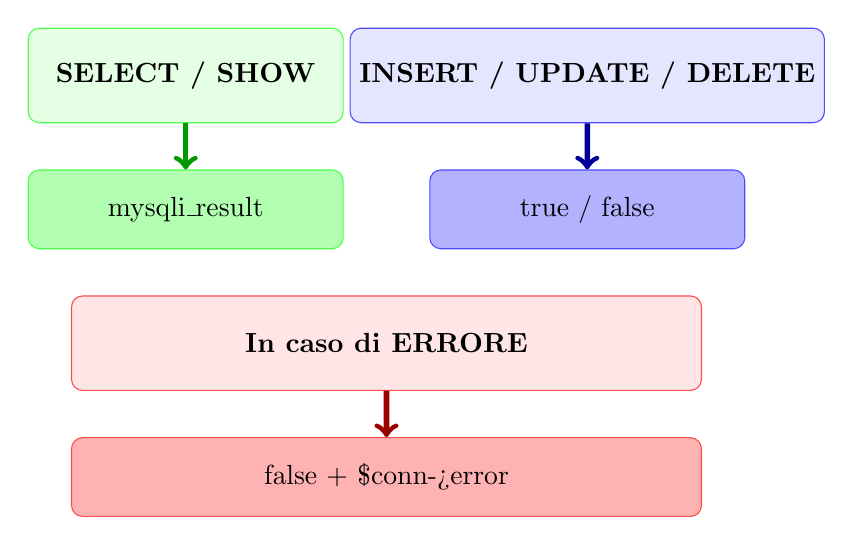
\begin{tikzpicture}[scale=0.85]
    % Query SELECT
    \node[rectangle,draw=green!70,fill=green!10,minimum width=4cm,minimum height=1.2cm,rounded corners] (select) at (0,3) {\textbf{SELECT / SHOW}};
    \node[rectangle,draw=green!70,fill=green!30,minimum width=4cm,minimum height=1cm,rounded corners] (selectr) at (0,1) {mysqli\_result};
    \draw[->,line width=2pt,green!60!black] (select) -- (selectr);
    
    % Query DML
    \node[rectangle,draw=blue!70,fill=blue!10,minimum width=4cm,minimum height=1.2cm,rounded corners] (dml) at (6,3) {\textbf{INSERT / UPDATE / DELETE}};
    \node[rectangle,draw=blue!70,fill=blue!30,minimum width=4cm,minimum height=1cm,rounded corners] (dmlr) at (6,1) {true / false};
    \draw[->,line width=2pt,blue!60!black] (dml) -- (dmlr);
    
    % Errore
    \node[rectangle,draw=red!70,fill=red!10,minimum width=8cm,minimum height=1.2cm,rounded corners] (error) at (3,-1) {\textbf{In caso di ERRORE}};
    \node[rectangle,draw=red!70,fill=red!30,minimum width=8cm,minimum height=1cm,rounded corners] (errorr) at (3,-3) {false + \$conn->error};
    \draw[->,line width=2pt,red!60!black] (error) -- (errorr);
\end{tikzpicture}
\end{center}
\end{frame}

% ====================
% SEZIONE 5: MYSQLI_RESULT
% ====================
\section{L'Oggetto mysqli\_result}

% ====================
% SLIDE 20
% ====================
\begin{frame}{L'Oggetto mysqli\_result}
\begin{block}{Definizione}
L'oggetto \texttt{mysqli\_result} rappresenta il risultato di una query eseguita su MySQL tramite l'estensione mysqli di PHP
\end{block}

\vspace{0.5cm}
\begin{center}
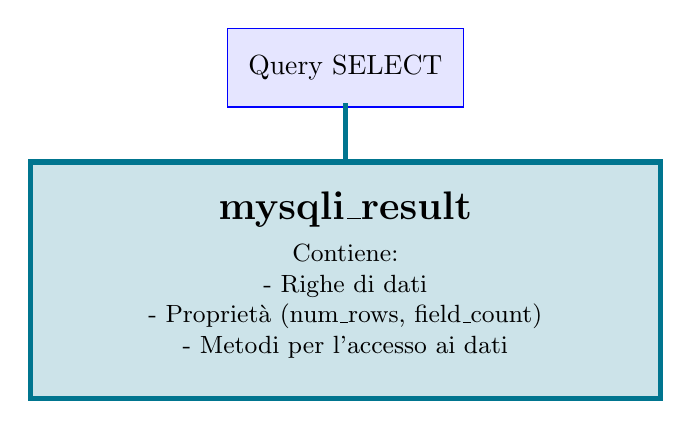
\begin{tikzpicture}[scale=0.9]
    % Query
    \node[rectangle,draw=blue,fill=blue!10,minimum width=3cm,minimum height=1cm] (query) at (0,3) {Query SELECT};
    
    % Freccia
    \draw[->,line width=2pt,mysqlblue] (0,2.5) -- (0,1.5);
    
    % mysqli_result
    \node[rectangle,draw=mysqlblue,fill=mysqlblue!20,minimum width=8cm,minimum height=3cm,line width=2pt] (result) at (0,0) {};
    \node[font=\Large\bfseries] at (0,1) {mysqli\_result};
    
    % Contenuto
    \node[font=\small,text width=7cm,align=center] at (0,-0.3) {
        Contiene:\\
        - Righe di dati\\
        - Proprietà (num\_rows, field\_count)\\
        - Metodi per l'accesso ai dati
    };
\end{tikzpicture}
\end{center}
\end{frame}

% ====================
% SLIDE 21
% ====================
\begin{frame}{Struttura mysqli\_result}
\begin{center}
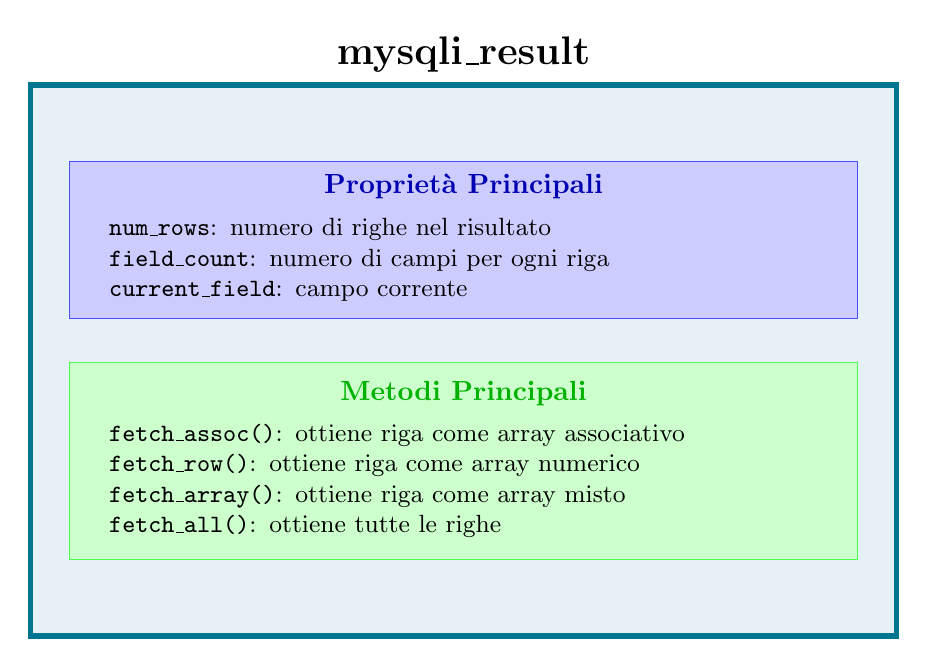
\begin{tikzpicture}[scale=0.85]
    % Box principale
    \node[rectangle,draw=mysqlblue,fill=mysqlblue!10,minimum width=11cm,minimum height=7cm,line width=2pt] (main) at (0,0) {};
    \node[above] at (main.north) {\Large\textbf{mysqli\_result}};
    
    % Proprietà
    \node[rectangle,draw=blue!70,fill=blue!20,minimum width=10cm,minimum height=2cm] (prop) at (0,1.8) {};
    \node[font=\bfseries,blue!70!black] at (0,2.6) {Proprietà Principali};
    \node[font=\small,text width=9cm,align=left] at (0,1.5) {
        \texttt{num\_rows}: numero di righe nel risultato\\
        \texttt{field\_count}: numero di campi per ogni riga\\
        \texttt{current\_field}: campo corrente
    };
    
    % Metodi
    \node[rectangle,draw=green!70,fill=green!20,minimum width=10cm,minimum height=2.5cm] (methods) at (0,-1.5) {};
    \node[font=\bfseries,green!70!black] at (0,-0.5) {Metodi Principali};
    \node[font=\small,text width=9cm,align=left] at (0,-1.8) {
        \texttt{fetch\_assoc()}: ottiene riga come array associativo\\
        \texttt{fetch\_row()}: ottiene riga come array numerico\\
        \texttt{fetch\_array()}: ottiene riga come array misto\\
        \texttt{fetch\_all()}: ottiene tutte le righe
    };
\end{tikzpicture}
\end{center}
\end{frame}

% ====================
% SLIDE 22
% ====================
\begin{frame}{Metodi Principali di mysqli\_result}
\begin{description}
    \item[fetch\_assoc()] Restituisce la riga corrente come array associativo
    \item[fetch\_row()] Restituisce la riga corrente come array numerico
    \item[fetch\_array()] Restituisce la riga corrente come array misto (associativo e numerico)
\end{description}

\vspace{0.5cm}
\begin{alertblock}{Comportamento}
Tutti questi metodi spostano automaticamente l'indicatore interno alla riga successiva dopo ogni chiamata
\end{alertblock}
\end{frame}

% ====================
% SLIDE 23
% ====================
\begin{frame}[fragile]{fetch\_assoc() - Array Associativo}
\begin{block}{Descrizione}
Restituisce un array associativo dove le chiavi sono i nomi dei campi
\end{block}

\begin{lstlisting}[style=phpstyle]
while($row = $result->fetch_assoc()) {
    echo "ID: " . $row["id"];
    echo " - Nome: " . $row["nome"];
    echo " - Cognome: " . $row["cognome"];
}
\end{lstlisting}

\vspace{0.3cm}
\begin{center}
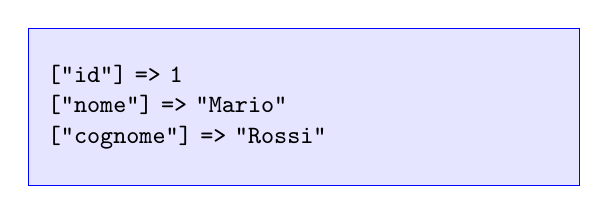
\begin{tikzpicture}[scale=0.7]
    \node[rectangle,draw=blue,fill=blue!10,minimum width=7cm,minimum height=2cm] (array) at (0,0) {};
    \node[font=\small,text width=6.5cm,align=left] at (0,0) {
        \texttt{["id"] => 1}\\
        \texttt{["nome"] => "Mario"}\\
        \texttt{["cognome"] => "Rossi"}
    };
\end{tikzpicture}
\end{center}

\vspace{0.2cm}
\begin{center}
\small\url{https://www.w3schools.com/php/func_mysqli_fetch_assoc.asp}
\end{center}
\end{frame}

% ====================
% SLIDE 24
% ====================
\begin{frame}[fragile]{Esempio Completo fetch\_assoc()}
\begin{lstlisting}[style=phpstyle]
<?php
$sql = "SELECT id, nome, cognome FROM studenti";
$result = $conn->query($sql);

if ($result->num_rows > 0) {
    // Output dei dati di ogni riga
    while($row = $result->fetch_assoc()) {
        echo "ID: " . $row["id"];
        echo " - Nome: " . $row["nome"];
        echo " - Cognome: " . $row["cognome"];
        echo "<br>";
    }
} else {
    echo "0 risultati";
}
?>
\end{lstlisting}
\end{frame}

% ====================
% SLIDE 25
% ====================
\begin{frame}[fragile]{fetch\_row() - Array Numerico}
\begin{block}{Descrizione}
Restituisce un array numerico dove gli indici sono posizionali (0, 1, 2, ...)
\end{block}

\begin{lstlisting}[style=phpstyle]
while($row = $result->fetch_row()) {
    echo "ID: " . $row[0];
    echo " - Nome: " . $row[1];
    echo " - Cognome: " . $row[2];
}
\end{lstlisting}

\vspace{0.3cm}
\begin{center}
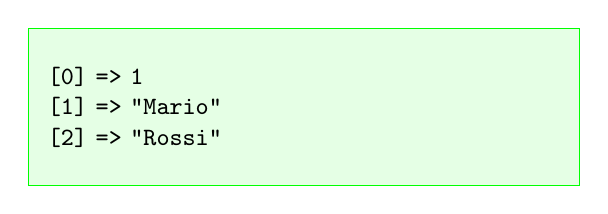
\begin{tikzpicture}[scale=0.7]
    \node[rectangle,draw=green,fill=green!10,minimum width=7cm,minimum height=2cm] (array) at (0,0) {};
    \node[font=\small,text width=6.5cm,align=left] at (0,0) {
        \texttt{[0] => 1}\\
        \texttt{[1] => "Mario"}\\
        \texttt{[2] => "Rossi"}
    };
\end{tikzpicture}
\end{center}

\vspace{0.2cm}
\begin{center}
\small\url{https://www.w3schools.com/php/func_mysqli_fetch_row.asp}
\end{center}
\end{frame}

% ====================
% SLIDE 26
% ====================
\begin{frame}[fragile]{Esempio Completo fetch\_row()}
\begin{lstlisting}[style=phpstyle]
<?php
$sql = "SELECT id, nome, cognome FROM studenti";
$result = $conn->query($sql);

if ($result->num_rows > 0) {
    // Output dei dati di ogni riga
    while($row = $result->fetch_row()) {
        echo "ID: " . $row[0];
        echo " - Nome: " . $row[1];
        echo " - Cognome: " . $row[2];
        echo "<br>";
    }
} else {
    echo "0 risultati";
}
?>
\end{lstlisting}
\end{frame}

% ====================
% SLIDE 27
% ====================
\begin{frame}[fragile]{Recuperare Tutte le Righe - fetch\_assoc()}
\begin{lstlisting}[style=phpstyle]
<?php
$sql = "SELECT id, nome, cognome FROM studenti";
$result = $conn->query($sql);

// Array per memorizzare tutti i risultati
$students = array();

while($row = $result->fetch_assoc()) {
    $students[] = $row;
}

// Utilizzo dell'array
foreach($students as $student) {
    echo $student["nome"] . " " . $student["cognome"];
    echo "<br>";
}
?>
\end{lstlisting}
\end{frame}

% ====================
% SLIDE 28
% ====================
\begin{frame}[fragile]{Recuperare Tutte le Righe - fetch\_row()}
\begin{lstlisting}[style=phpstyle]
<?php
$sql = "SELECT id, nome, cognome FROM studenti";
$result = $conn->query($sql);

// Array per memorizzare tutti i risultati
$students = array();

while($row = $result->fetch_row()) {
    $students[] = $row;
}

// Utilizzo dell'array
foreach($students as $student) {
    echo $student[1] . " " . $student[2];
    echo "<br>";
}
?>
\end{lstlisting}
\end{frame}

% ====================
% SLIDE 29
% ====================
\begin{frame}{Il Metodo fetch\_all()}
\begin{block}{Descrizione}
Il metodo \texttt{fetch\_all()} restituisce TUTTE le righe del risultato in un unico array bidimensionale
\end{block}

\vspace{0.3cm}
\textbf{Parametri:}
\begin{description}
    \item[resulttype] (opzionale) Specifica il tipo di array:
    \begin{itemize}
        \item \texttt{MYSQLI\_ASSOC} - Array associativo (default)
        \item \texttt{MYSQLI\_NUM} - Array numerico
        \item \texttt{MYSQLI\_BOTH} - Entrambi i tipi
    \end{itemize}
\end{description}

\vspace{0.3cm}
\begin{alertblock}{Vantaggio}
Operazione più veloce rispetto al ciclo while con fetch\_assoc/fetch\_row
\end{alertblock}
\end{frame}

% ====================
% SLIDE 30
% ====================
\begin{frame}[fragile]{Esempio fetch\_all() - Base}
\begin{lstlisting}[style=phpstyle]
<?php
$sql = "SELECT id, nome, cognome FROM studenti";
$result = $conn->query($sql);

// Ottiene tutte le righe in un colpo solo
$students = $result->fetch_all();

// Visualizzazione
foreach($students as $student) {
    print_r($student);
    echo "<br>";
}
?>
\end{lstlisting}
\end{frame}

% ====================
% SLIDE 31
% ====================
\begin{frame}[fragile]{fetch\_all() - Utilizzo Pratico}
\begin{lstlisting}[style=phpstyle]
<?php
$sql = "SELECT id, nome, cognome FROM studenti";
$result = $conn->query($sql);

if ($result->num_rows > 0) {
    $all_data = $result->fetch_all(MYSQLI_ASSOC);
    
    echo "<table border='1'>";
    echo "<tr><th>ID</th><th>Nome</th><th>Cognome</th></tr>";
    
    foreach($all_data as $row) {
        echo "<tr>";
        echo "<td>" . $row["id"] . "</td>";
        echo "<td>" . $row["nome"] . "</td>";
        echo "<td>" . $row["cognome"] . "</td>";
        echo "</tr>";
    }
    echo "</table>";
}
?>
\end{lstlisting}
\end{frame}

% ====================
% SLIDE 32
% ====================
\begin{frame}{fetch\_all(MYSQLI\_ASSOC)}
\begin{center}
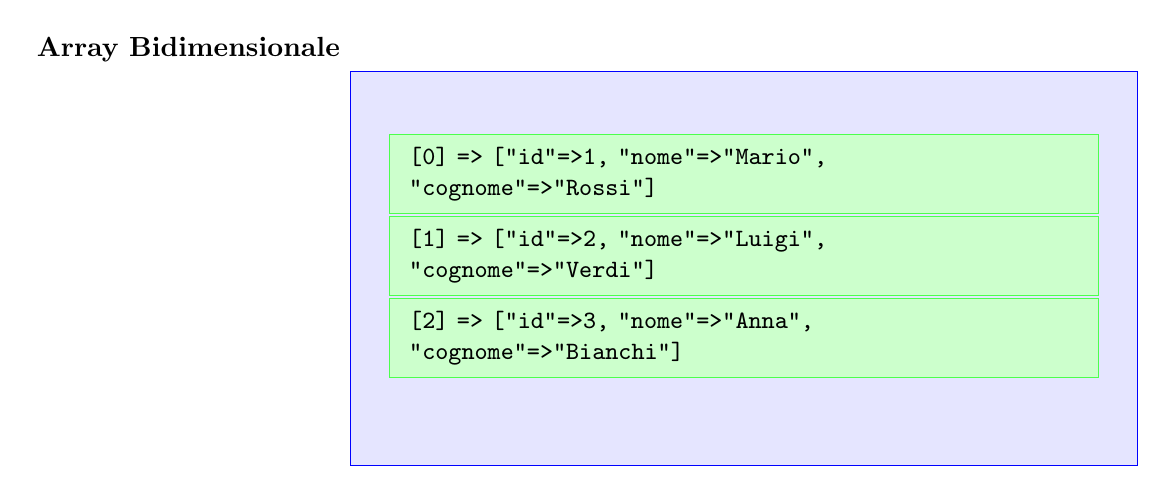
\begin{tikzpicture}[scale=0.8]
    % Array esterno
    \node[rectangle,draw=blue,fill=blue!10,minimum width=10cm,minimum height=5cm] (main) at (0,0) {};
    \node[above left] at (main.north west) {\textbf{Array Bidimensionale}};
    
    % Riga 0
    \node[rectangle,draw=green!70,fill=green!20,minimum width=9cm,minimum height=1cm] (row0) at (0,1.5) {};
    \node[font=\small,text width=8.5cm,align=left] at (0,1.5) {
        \texttt{[0] => ["id"=>1, "nome"=>"Mario", "cognome"=>"Rossi"]}
    };
    
    % Riga 1
    \node[rectangle,draw=green!70,fill=green!20,minimum width=9cm,minimum height=1cm] (row1) at (0,0.2) {};
    \node[font=\small,text width=8.5cm,align=left] at (0,0.2) {
        \texttt{[1] => ["id"=>2, "nome"=>"Luigi", "cognome"=>"Verdi"]}
    };
    
    % Riga 2
    \node[rectangle,draw=green!70,fill=green!20,minimum width=9cm,minimum height=1cm] (row2) at (0,-1.1) {};
    \node[font=\small,text width=8.5cm,align=left] at (0,-1.1) {
        \texttt{[2] => ["id"=>3, "nome"=>"Anna", "cognome"=>"Bianchi"]}
    };
\end{tikzpicture}
\end{center}
\end{frame}

% ====================
% SLIDE 33
% ====================
\begin{frame}{fetch\_all(MYSQLI\_ASSOC) - Caratteristiche}
\begin{block}{Struttura}
Restituisce un array bidimensionale dove:
\begin{itemize}
    \item Il primo livello ha indici numerici (0, 1, 2, ...)
    \item Il secondo livello ha chiavi associative (nomi dei campi)
\end{itemize}
\end{block}

\vspace{0.5cm}
\textbf{Accesso ai dati:}
\begin{center}
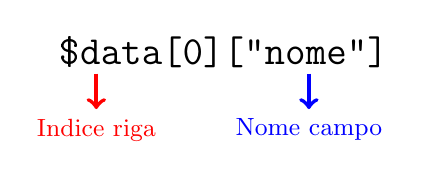
\begin{tikzpicture}[scale=0.9]
    \node[font=\Large\ttfamily] at (0,0) {\$data[0]["nome"]};
    \draw[->,red,line width=1.5pt] (-1.8,-0.3) -- (-1.8,-0.8);
    \node[red,font=\small,below] at (-1.8,-0.8) {Indice riga};
    \draw[->,blue,line width=1.5pt] (1.2,-0.3) -- (1.2,-0.8);
    \node[blue,font=\small,below] at (1.2,-0.8) {Nome campo};
\end{tikzpicture}
\end{center}
\end{frame}

% ====================
% SLIDE 34
% ====================
\begin{frame}{fetch\_all(MYSQLI\_NUM)}
\begin{center}
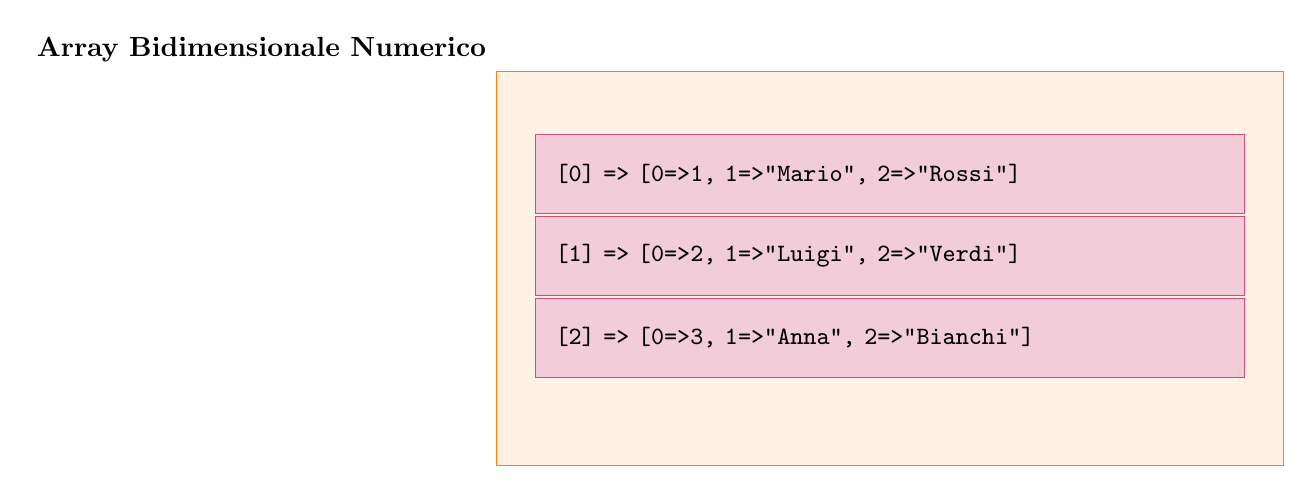
\begin{tikzpicture}[scale=0.8]
    % Array esterno
    \node[rectangle,draw=orange,fill=orange!10,minimum width=10cm,minimum height=5cm] (main) at (0,0) {};
    \node[above left] at (main.north west) {\textbf{Array Bidimensionale Numerico}};
    
    % Riga 0
    \node[rectangle,draw=purple!70,fill=purple!20,minimum width=9cm,minimum height=1cm] (row0) at (0,1.5) {};
    \node[font=\small,text width=8.5cm,align=left] at (0,1.5) {
        \texttt{[0] => [0=>1, 1=>"Mario", 2=>"Rossi"]}
    };
    
    % Riga 1
    \node[rectangle,draw=purple!70,fill=purple!20,minimum width=9cm,minimum height=1cm] (row1) at (0,0.2) {};
    \node[font=\small,text width=8.5cm,align=left] at (0,0.2) {
        \texttt{[1] => [0=>2, 1=>"Luigi", 2=>"Verdi"]}
    };
    
    % Riga 2
    \node[rectangle,draw=purple!70,fill=purple!20,minimum width=9cm,minimum height=1cm] (row2) at (0,-1.1) {};
    \node[font=\small,text width=8.5cm,align=left] at (0,-1.1) {
        \texttt{[2] => [0=>3, 1=>"Anna", 2=>"Bianchi"]}
    };
\end{tikzpicture}
\end{center}
\end{frame}

% ====================
% SLIDE 35
% ====================
\begin{frame}{fetch\_all(MYSQLI\_NUM) - Caratteristiche}
\begin{block}{Struttura}
Restituisce un array bidimensionale dove:
\begin{itemize}
    \item ENTRAMBI i livelli hanno indici numerici
    \item Accesso più veloce ma meno leggibile
\end{itemize}
\end{block}

\vspace{0.5cm}
\textbf{Accesso ai dati:}
\begin{center}
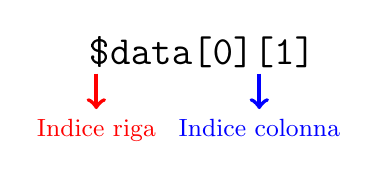
\begin{tikzpicture}[scale=0.9]
    \node[font=\Large\ttfamily] at (0,0) {\$data[0][1]};
    \draw[->,red,line width=1.5pt] (-1.5,-0.3) -- (-1.5,-0.8);
    \node[red,font=\small,below] at (-1.5,-0.8) {Indice riga};
    \draw[->,blue,line width=1.5pt] (0.8,-0.3) -- (0.8,-0.8);
    \node[blue,font=\small,below] at (0.8,-0.8) {Indice colonna};
\end{tikzpicture}
\end{center}
\end{frame}

% ====================
% SLIDE 36
% ====================
\begin{frame}[fragile]{Il Metodo close()}
\begin{block}{Descrizione}
Il metodo \texttt{close()} chiude la connessione al database MySQL
\end{block}

\vspace{0.3cm}
\textbf{Parametri:}
\begin{itemize}
    \item Nessun parametro richiesto
\end{itemize}

\vspace{0.3cm}
\textbf{Valori Restituiti:}
\begin{itemize}
    \item \texttt{true} in caso di successo
    \item \texttt{false} in caso di errore
\end{itemize}

\vspace{0.3cm}
\begin{lstlisting}[style=phpstyle]
// Chiusura della connessione
$conn->close();
\end{lstlisting}
\end{frame}

% ====================
% SLIDE 37
% ====================
\begin{frame}[fragile]{La Proprietà num\_rows}
\begin{block}{Descrizione}
Rappresenta il numero di righe nel risultato di una query SELECT
\end{block}

\vspace{0.3cm}
\begin{lstlisting}[style=phpstyle]
$sql = "SELECT * FROM studenti";
$result = $conn->query($sql);

echo "Numero di record trovati: " . $result->num_rows;

if ($result->num_rows > 0) {
    // Processa i risultati
    while($row = $result->fetch_assoc()) {
        echo $row["nome"];
    }
} else {
    echo "Nessun risultato trovato";
}
\end{lstlisting}
\end{frame}

% ====================
% SEZIONE 6: CRUD
% ====================
\section{Operazioni CRUD}

% ====================
% SLIDE 38
% ====================
\begin{frame}{Operazioni CRUD}
\begin{center}
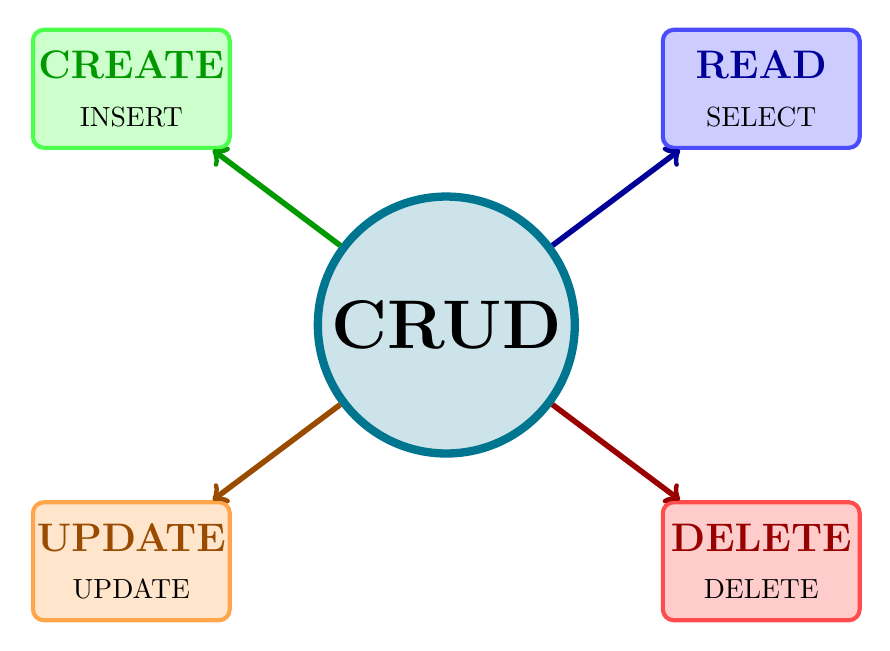
\begin{tikzpicture}[scale=1]
    % CRUD al centro
    \node[circle,draw=mysqlblue,fill=mysqlblue!20,minimum size=2.5cm,line width=3pt,font=\Huge\bfseries] (crud) at (0,0) {CRUD};
    
    % Create
    \node[rectangle,draw=green!70,fill=green!20,minimum width=2.5cm,minimum height=1.5cm,rounded corners,line width=1.5pt] (create) at (-4,3) {};
    \node[font=\Large\bfseries,green!60!black] at (create.north) [below=5pt] {CREATE};
    \node[font=\normalsize] at (create.south) [above=5pt] {INSERT};
    
    % Read
    \node[rectangle,draw=blue!70,fill=blue!20,minimum width=2.5cm,minimum height=1.5cm,rounded corners,line width=1.5pt] (read) at (4,3) {};
    \node[font=\Large\bfseries,blue!60!black] at (read.north) [below=5pt] {READ};
    \node[font=\normalsize] at (read.south) [above=5pt] {SELECT};
    
    % Update
    \node[rectangle,draw=orange!70,fill=orange!20,minimum width=2.5cm,minimum height=1.5cm,rounded corners,line width=1.5pt] (update) at (-4,-3) {};
    \node[font=\Large\bfseries,orange!60!black] at (update.north) [below=5pt] {UPDATE};
    \node[font=\normalsize] at (update.south) [above=5pt] {UPDATE};
    
    % Delete
    \node[rectangle,draw=red!70,fill=red!20,minimum width=2.5cm,minimum height=1.5cm,rounded corners,line width=1.5pt] (delete) at (4,-3) {};
    \node[font=\Large\bfseries,red!60!black] at (delete.north) [below=5pt] {DELETE};
    \node[font=\normalsize] at (delete.south) [above=5pt] {DELETE};
    
    % Connessioni
    \draw[->,line width=2pt,green!60!black] (crud) -- (create);
    \draw[->,line width=2pt,blue!60!black] (crud) -- (read);
    \draw[->,line width=2pt,orange!60!black] (crud) -- (update);
    \draw[->,line width=2pt,red!60!black] (crud) -- (delete);
\end{tikzpicture}
\end{center}
\end{frame}

% ====================
% SLIDE 39
% ====================
\begin{frame}[fragile]{Inserimento Record - INSERT}
\begin{block}{Sintassi SQL}
\begin{lstlisting}[style=sqlstyle]
INSERT INTO nome_tabella (campo1, campo2, campo3)
VALUES (valore1, valore2, valore3);
\end{lstlisting}
\end{block}

\vspace{0.3cm}
\textbf{Esempio in PHP:}
\begin{lstlisting}[style=phpstyle]
$nome = "Mario";
$cognome = "Rossi";
$email = "mario.rossi@email.com";

$sql = "INSERT INTO studenti (nome, cognome, email)
        VALUES ('$nome', '$cognome', '$email')";

if ($conn->query($sql) === TRUE) {
    echo "Nuovo record inserito con successo";
} else {
    echo "Errore: " . $conn->error;
}
\end{lstlisting}
\end{frame}

% ====================
% SLIDE 40
% ====================
\begin{frame}[fragile]{Aggiornamento Dati - UPDATE}
\begin{block}{Sintassi SQL}
\begin{lstlisting}[style=sqlstyle]
UPDATE nome_tabella
SET campo1 = valore1, campo2 = valore2
WHERE condizione;
\end{lstlisting}
\end{block}

\vspace{0.3cm}
\textbf{Esempio in PHP:}
\begin{lstlisting}[style=phpstyle]
$id = 5;
$nuovo_email = "nuova.email@domain.com";

$sql = "UPDATE studenti 
        SET email = '$nuovo_email' 
        WHERE id = $id";

if ($conn->query($sql) === TRUE) {
    echo "Record aggiornato con successo";
} else {
    echo "Errore: " . $conn->error;
}
\end{lstlisting}
\end{frame}

% ====================
% SLIDE 41
% ====================
\begin{frame}[fragile]{Cancellazione Record - DELETE}
\begin{block}{Sintassi SQL}
\begin{lstlisting}[style=sqlstyle]
DELETE FROM nome_tabella WHERE condizione;
\end{lstlisting}
\end{block}

\vspace{0.3cm}
\textbf{Esempio in PHP:}
\begin{lstlisting}[style=phpstyle]
$id_da_cancellare = 5;

$sql = "DELETE FROM studenti WHERE id = $id_da_cancellare";

if ($conn->query($sql) === TRUE) {
    echo "Record cancellato con successo";
} else {
    echo "Errore: " . $conn->error;
}
\end{lstlisting}

\vspace{0.3cm}
\begin{alertblock}{ATTENZIONE!}
Fare sempre attenzione alla clausola WHERE per evitare cancellazioni accidentali
\end{alertblock}
\end{frame}

% ====================
% SEZIONE 7: PREPARED STATEMENTS
% ====================
\section{Prepared Statements}

% ====================
% SLIDE 42
% ====================
\begin{frame}{Ottimizzazioni e Sicurezza}
\begin{center}
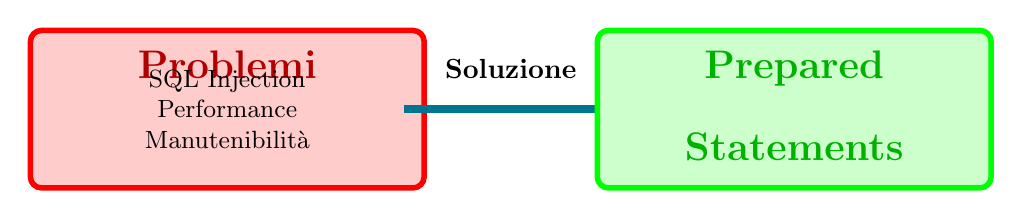
\begin{tikzpicture}[scale=0.9]
    % Problema
    \node[rectangle,draw=red,fill=red!20,minimum width=5cm,minimum height=2cm,rounded corners,line width=2pt] (prob) at (-4,0) {};
    \node[font=\Large\bfseries,red!70!black] at (prob.north) [below=5pt] {Problemi};
    \node[font=\small,text width=4.5cm,align=center] at (prob.center) {
        SQL Injection\\
        Performance\\
        Manutenibilità
    };
    
    % Freccia
    \draw[->,line width=3pt,mysqlblue] (-1.5,0) -- (1.5,0);
    \node[above,font=\bfseries] at (0,0.3) {Soluzione};
    
    % Soluzione
    \node[rectangle,draw=green,fill=green!20,minimum width=5cm,minimum height=2cm,rounded corners,line width=2pt] (sol) at (4,0) {};
    \node[font=\Large\bfseries,green!70!black] at (sol.north) [below=5pt] {Prepared};
    \node[font=\Large\bfseries,green!70!black] at (sol.center) [below=5pt] {Statements};
\end{tikzpicture}
\end{center}
\end{frame}

% ====================
% SLIDE 43
% ====================
\begin{frame}{Metodi prepare() e bind\_param()}
\begin{block}{Introduzione}
L'utilizzo di \texttt{prepare()} e \texttt{bind\_param()} rappresenta una best practice per:
\begin{itemize}
    \item Sicurezza (prevenzione SQL injection)
    \item Performance (ottimizzazione delle query)
    \item Manutenibilità del codice
\end{itemize}
\end{block}

\vspace{0.5cm}
\begin{center}
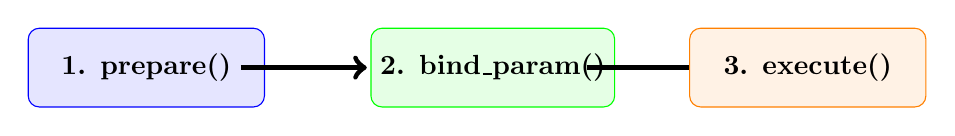
\begin{tikzpicture}[scale=0.8]
    \node[rectangle,draw=blue,fill=blue!10,rounded corners,minimum width=3cm,minimum height=1cm] (p1) at (0,0) {\textbf{1. prepare()}};
    \draw[->,line width=2pt] (1.5,0) -- (3.5,0);
    \node[rectangle,draw=green,fill=green!10,rounded corners,minimum width=3cm,minimum height=1cm] (p2) at (5.5,0) {\textbf{2. bind\_param()}};
    \draw[->,line width=2pt] (7,0) -- (9,0);
    \node[rectangle,draw=orange,fill=orange!10,rounded corners,minimum width=3cm,minimum height=1cm] (p3) at (10.5,0) {\textbf{3. execute()}};
\end{tikzpicture}
\end{center}
\end{frame}

% ====================
% SLIDE 44
% ====================
\begin{frame}{Prevenzione SQL Injection}
\begin{block}{Parametri Disassociati dalla Query}
Con \texttt{prepare()} e \texttt{bind\_param()}, i dati vengono separati dalle istruzioni SQL
\end{block}

\vspace{0.3cm}
\begin{center}
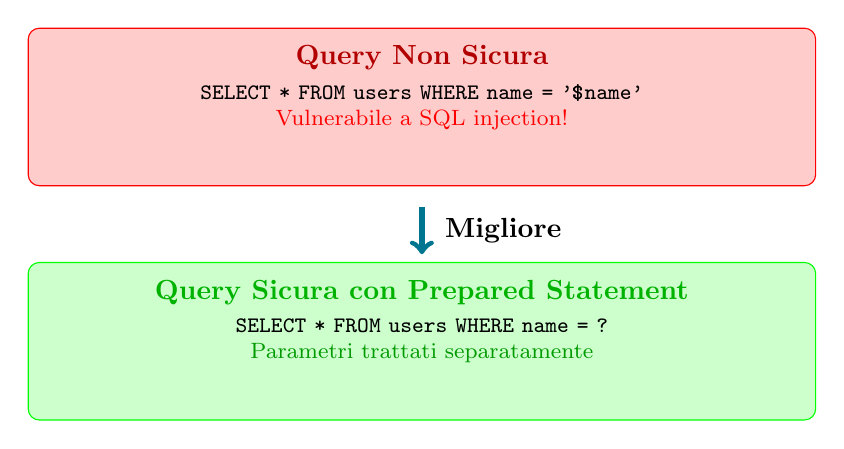
\begin{tikzpicture}[scale=0.85]
    % Query non sicura
    \node[rectangle,draw=red,fill=red!20,minimum width=10cm,minimum height=2cm,rounded corners] (unsafe) at (0,2) {};
    \node[font=\bfseries,red!70!black] at (unsafe.north) [below=3pt] {Query Non Sicura};
    \node[font=\footnotesize,text width=9.5cm,align=center] at (unsafe.center) {
        \texttt{SELECT * FROM users WHERE name = '\$name'} \\
        {\color{red}Vulnerabile a SQL injection!}
    };
    
    % Query sicura
    \node[rectangle,draw=green,fill=green!20,minimum width=10cm,minimum height=2cm,rounded corners] (safe) at (0,-1.5) {};
    \node[font=\bfseries,green!70!black] at (safe.north) [below=3pt] {Query Sicura con Prepared Statement};
    \node[font=\footnotesize,text width=9.5cm,align=center] at (safe.center) {
        \texttt{SELECT * FROM users WHERE name = ?} \\
        {\color{green!60!black}Parametri trattati separatamente}
    };
    
    \draw[->,line width=2pt,mysqlblue] (0,0.5) -- (0,-0.2);
    \node[right,font=\bfseries] at (0.2,0.15) {Migliore};
\end{tikzpicture}
\end{center}
\end{frame}

% ====================
% SLIDE 45
% ====================
\begin{frame}{Prestazioni Ottimizzate}
\begin{block}{Caching del Piano di Esecuzione}
La preparazione di una query consente al database di:
\begin{itemize}
    \item Analizzare la query una sola volta
    \item Ottimizzare il piano di esecuzione
    \item Memorizzare in cache il piano
    \item Riutilizzare lo stesso piano con parametri diversi
\end{itemize}
\end{block}

\vspace{0.3cm}
\begin{center}
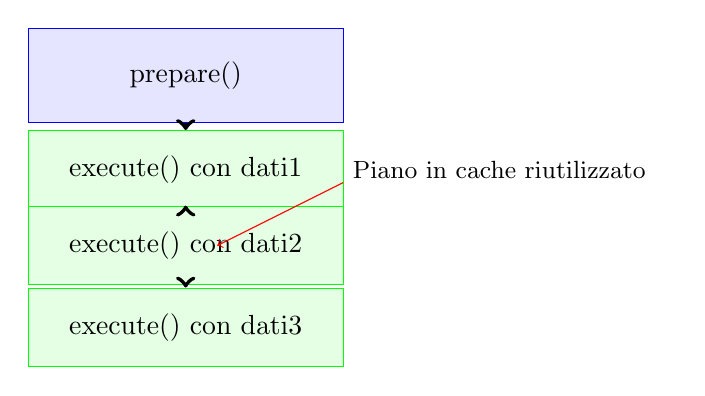
\begin{tikzpicture}[scale=0.8]
    % Prima esecuzione
    \node[rectangle,draw=blue,fill=blue!10,minimum width=4cm,minimum height=1.2cm] (p1) at (0,2) {prepare()};
    \node[rectangle,draw=green,fill=green!10,minimum width=4cm,minimum height=1cm] (e1) at (0,0.5) {execute() con dati1};
    
    % Esecuzioni successive
    \node[rectangle,draw=green,fill=green!10,minimum width=4cm,minimum height=1cm] (e2) at (0,-0.7) {execute() con dati2};
    \node[rectangle,draw=green,fill=green!10,minimum width=4cm,minimum height=1cm] (e3) at (0,-2) {execute() con dati3};
    
    % Annotazioni
    \draw[->,line width=1.5pt] (p1) -- (e1);
    \draw[->,line width=1.5pt,dashed] (e1) -- (e2);
    \draw[->,line width=1.5pt,dashed] (e2) -- (e3);
    
    \node[right,font=\small,text width=4cm] at (2.5,0.5) {Piano in cache riutilizzato};
    \draw[->,red] (2.5,0.3) -- (0.5,-0.7);
\end{tikzpicture}
\end{center}
\end{frame}

% ====================
% SLIDE 46
% ====================
\begin{frame}{Leggibilità del Codice}
\begin{block}{Separazione Struttura e Dati}
L'utilizzo di segnaposto rende il codice più:
\begin{itemize}
    \item Leggibile
    \item Manutenibile
    \item Comprensibile
\end{itemize}
\end{block}

\vspace{0.5cm}
\begin{center}
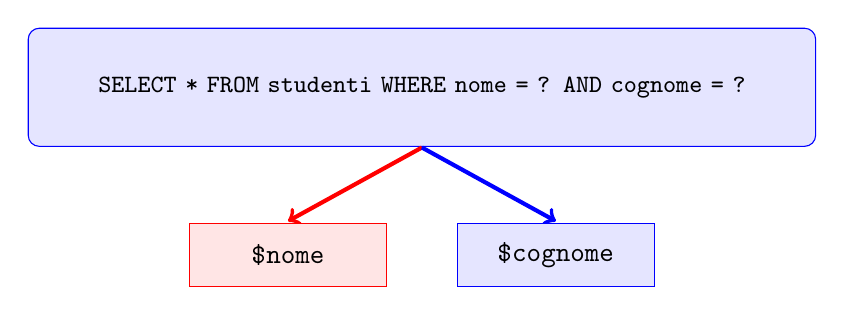
\begin{tikzpicture}[scale=0.85]
    % Query con segnaposto
    \node[rectangle,draw=blue,fill=blue!10,minimum width=10cm,minimum height=1.5cm,rounded corners] (query) at (0,0) {};
    \node[font=\small,text width=9.5cm,align=center] at (query.center) {
        \texttt{SELECT * FROM studenti WHERE nome = ? AND cognome = ?}
    };
    
    % Frecce verso i dati
    \draw[->,line width=1.5pt,red] (0,-0.9) -- (-2,-2);
    \draw[->,line width=1.5pt,blue] (0,-0.9) -- (2,-2);
    
    % Dati
    \node[rectangle,draw=red,fill=red!10,minimum width=2.5cm,minimum height=0.8cm] (d1) at (-2,-2.5) {\texttt{\$nome}};
    \node[rectangle,draw=blue,fill=blue!10,minimum width=2.5cm,minimum height=0.8cm] (d2) at (2,-2.5) {\texttt{\$cognome}};
\end{tikzpicture}
\end{center}
\end{frame}

% ====================
% SLIDE 47
% ====================

\vspace{0.3cm}
\begin{frame}
\begin{center}
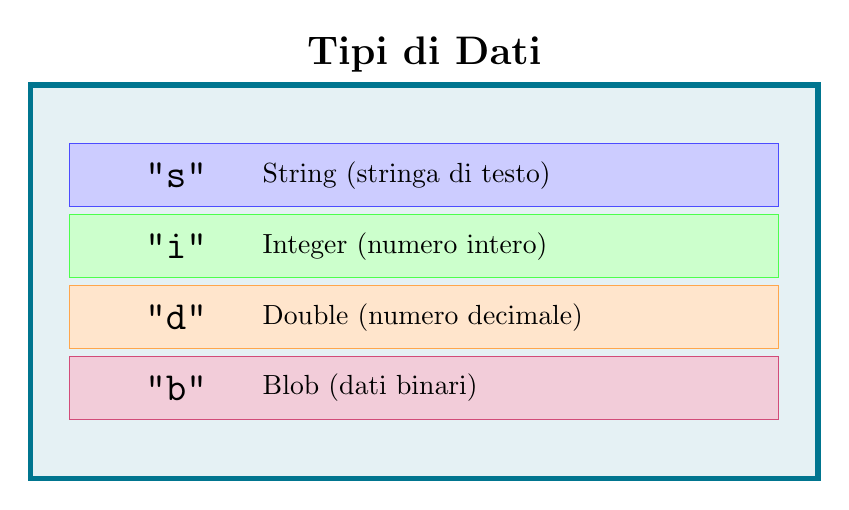
\begin{tikzpicture}[scale=0.9]
    % Tabella dei tipi
    \node[rectangle,draw=mysqlblue,fill=mysqlblue!10,minimum width=10cm,minimum height=5cm,line width=2pt] (main) at (0,0) {};
    \node[above] at (main.north) {\Large\bfseries Tipi di Dati};
    
    % Tipo s
    \node[rectangle,draw=blue!70,fill=blue!20,minimum width=9cm,minimum height=0.8cm] (s) at (0,1.5) {};
    \node[font=\Large\bfseries\ttfamily] at (-3.5,1.5) {"s"};
    \node[font=\normalsize,text width=5cm,align=left] at (0.5,1.5) {String (stringa di testo)};
    
    % Tipo i
    \node[rectangle,draw=green!70,fill=green!20,minimum width=9cm,minimum height=0.8cm] (i) at (0,0.5) {};
    \node[font=\Large\bfseries\ttfamily] at (-3.5,0.5) {"i"};
    \node[font=\normalsize,text width=5cm,align=left] at (0.5,0.5) {Integer (numero intero)};
    
    % Tipo d
    \node[rectangle,draw=orange!70,fill=orange!20,minimum width=9cm,minimum height=0.8cm] (d) at (0,-0.5) {};
    \node[font=\Large\bfseries\ttfamily] at (-3.5,-0.5) {"d"};
    \node[font=\normalsize,text width=5cm,align=left] at (0.5,-0.5) {Double (numero decimale)};
    
    % Tipo b
    \node[rectangle,draw=purple!70,fill=purple!20,minimum width=9cm,minimum height=0.8cm] (b) at (0,-1.5) {};
    \node[font=\Large\bfseries\ttfamily] at (-3.5,-1.5) {"b"};
    \node[font=\normalsize,text width=5cm,align=left] at (0.5,-1.5) {Blob (dati binari)};
\end{tikzpicture}
\end{center}
\end{frame}

% ====================
% SLIDE 48
% ====================
\begin{frame}{Compatibilità con Database Diversi}
\begin{center}
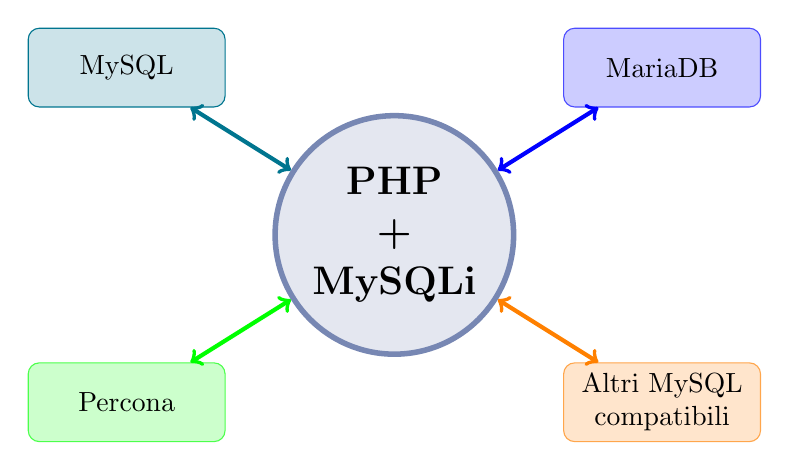
\begin{tikzpicture}[scale=0.85]
    % PHP al centro
    \node[circle,draw=phpblue,fill=phpblue!20,minimum size=2.5cm,line width=2pt,font=\Large\bfseries,align=center] (php) at (0,0) {PHP \\ + \\ MySQLi};
    
    % Database supportati
    \node[rectangle,draw=mysqlblue,fill=mysqlblue!20,minimum width=2.5cm,minimum height=1cm,rounded corners] (mysql) at (-4,2.5) {MySQL};
    
    \node[rectangle,draw=blue!70,fill=blue!20,minimum width=2.5cm,minimum height=1cm,rounded corners] (maria) at (4,2.5) {MariaDB};
    
    \node[rectangle,draw=green!70,fill=green!20,minimum width=2.5cm,minimum height=1cm,rounded corners] (perc) at (-4,-2.5) {Percona};
    
    \node[rectangle,draw=orange!70,fill=orange!20,minimum width=2.5cm,minimum height=1cm,rounded corners,align=center] (other) at (4,-2.5) {Altri MySQL\\compatibili};
    
    % Connessioni
    \draw[<->,line width=1.5pt,mysqlblue] (php) -- (mysql);
    \draw[<->,line width=1.5pt,blue] (php) -- (maria);
    \draw[<->,line width=1.5pt,green] (php) -- (perc);
    \draw[<->,line width=1.5pt,orange] (php) -- (other);
\end{tikzpicture}
\end{center}
\end{frame}

% ====================
% SLIDE 49
% ====================
\begin{frame}{Il Metodo prepare()}
\begin{block}{Descrizione}
Il metodo \texttt{prepare()} prepara una query SQL per l'esecuzione, creando un piano di esecuzione ottimizzato
\end{block}

\vspace{0.5cm}
\begin{center}
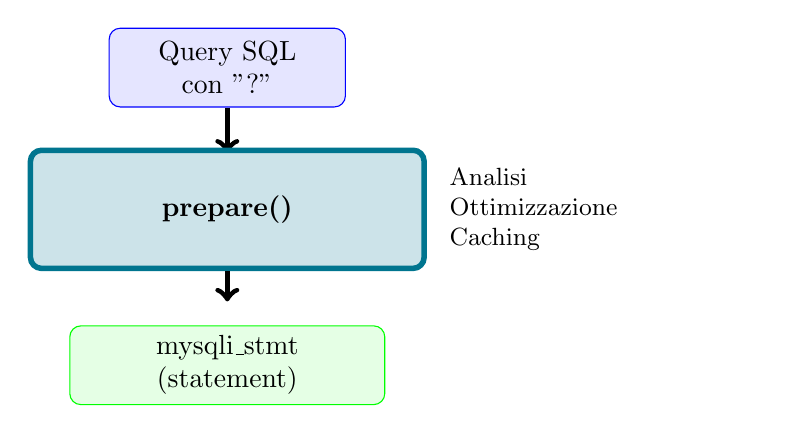
\begin{tikzpicture}[scale=0.9]
    % Flusso del prepare
    \node[rectangle,draw=blue,fill=blue!10,minimum width=3cm,minimum height=1cm,rounded corners,align=center] (query) at (0,3) {Query SQL \\ con "?"};
    
    \draw[->,line width=2pt] (query) -- (0,1.8);
    
    \node[rectangle,draw=mysqlblue,fill=mysqlblue!20,minimum width=5cm,minimum height=1.5cm,rounded corners,line width=2pt] (prepare) at (0,1) {\textbf{prepare()}};
    
    \draw[->,line width=2pt] (prepare) -- (0,-0.3);
    
    \node[rectangle,draw=green,fill=green!10,minimum width=4cm,minimum height=1cm,rounded corners,align=center] (stmt) at (0,-1.2) {mysqli\_stmt \\ (statement)};
    
    % Annotazioni
    \node[right,font=\small,text width=4cm,align=left] at (3,1) {Analisi \\ Ottimizzazione \\ Caching};
\end{tikzpicture}
\end{center}
\end{frame}

% ====================
% SLIDE 50
% ====================
\begin{frame}{Metodo prepare() - Parametri e Ritorno}
\begin{block}{Parametri}
\begin{description}
    \item[Query (string)] La query SQL da preparare, contenente segnaposto "?" per i parametri
    \item[Connessione] L'oggetto mysqli di connessione al database
\end{description}
\end{block}

\vspace{0.5cm}
\begin{block}{Valori di Ritorno}
Restituisce un oggetto di tipo \texttt{mysqli\_stmt} (statement) che rappresenta la query preparata
\end{block}

\vspace{0.3cm}
\begin{alertblock}{NOTA}
Il segnaposto "?" viene successivamente sostituito con i valori reali tramite \texttt{bind\_param()}
\end{alertblock}
\end{frame}

% ====================
% SLIDE 51
% ====================
\begin{frame}[fragile]{Esempio Metodo prepare()}
\begin{lstlisting}[style=phpstyle]
<?php
// Query con segnaposto
$sql = "SELECT id, nome, cognome FROM studenti 
        WHERE cognome = ? AND anno = ?";

// Preparazione della query
$stmt = $conn->prepare($sql);

if ($stmt === false) {
    die("Errore nella preparazione: " . $conn->error);
}

A questo punto la query è pronta per il binding dei parametri
 e l'esecuzione
?>
\end{lstlisting}
\end{frame}

% ====================
% SLIDE 52
% ====================
\begin{frame}{L'Oggetto mysqli\_stmt}
\begin{center}
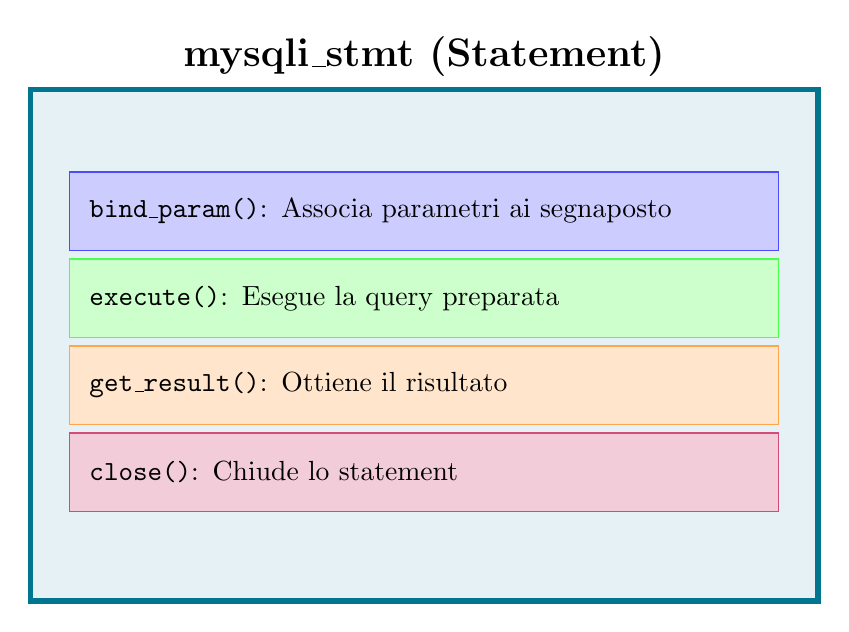
\begin{tikzpicture}[scale=0.85]
    % Box principale
    \node[rectangle,draw=mysqlblue,fill=mysqlblue!10,minimum width=10cm,minimum height=6.5cm,line width=2pt] (main) at (0,0) {};
    \node[above] at (main.north) {\Large\bfseries mysqli\_stmt (Statement)};
    
    % Metodi principali
    \node[rectangle,draw=blue!70,fill=blue!20,minimum width=9cm,minimum height=1cm] (bind) at (0,2) {};
    \node[font=\normalsize,text width=8.5cm,align=left] at (0,2) {
        \texttt{bind\_param()}: Associa parametri ai segnaposto
    };
    
    \node[rectangle,draw=green!70,fill=green!20,minimum width=9cm,minimum height=1cm] (exec) at (0,0.7) {};
    \node[font=\normalsize,text width=8.5cm,align=left] at (0,0.7) {
        \texttt{execute()}: Esegue la query preparata
    };
    
    \node[rectangle,draw=orange!70,fill=orange!20,minimum width=9cm,minimum height=1cm] (result) at (0,-0.6) {};
    \node[font=\normalsize,text width=8.5cm,align=left] at (0,-0.6) {
        \texttt{get\_result()}: Ottiene il risultato
    };
    
    \node[rectangle,draw=purple!70,fill=purple!20,minimum width=9cm,minimum height=1cm] (close) at (0,-1.9) {};
    \node[font=\normalsize,text width=8.5cm,align=left] at (0,-1.9) {
        \texttt{close()}: Chiude lo statement
    };
\end{tikzpicture}
\end{center}
\end{frame}

% ====================
% SLIDE 53
% ====================
\begin{frame}{Il Metodo bind\_param()}
\begin{block}{Descrizione}
Il metodo \texttt{bind\_param()} sostituisce i segnaposto "?" con i valori reali
\end{block}

\vspace{0.3cm}
\begin{center}
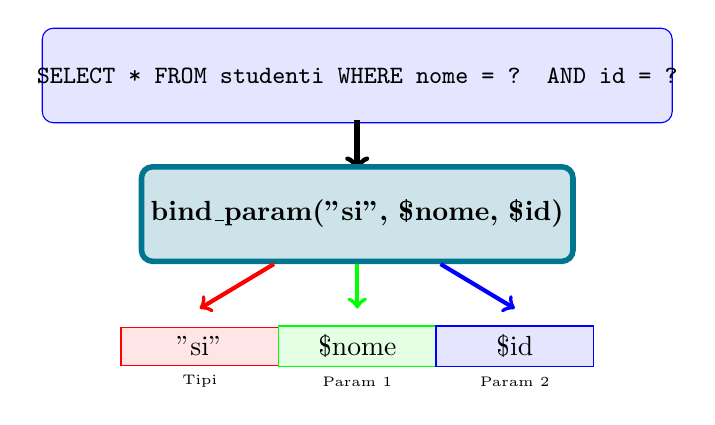
\begin{tikzpicture}[scale=0.8]
    % Query preparata
    \node[rectangle,draw=blue,fill=blue!10,minimum width=8cm,minimum height=1.2cm,rounded corners] (query) at (0,2.5) {};
    \node[font=\small] at (0,2.5) {\texttt{SELECT * FROM studenti WHERE nome = ? AND id = ?}};
    
    % bind_param
    \draw[->,line width=2pt] (0,1.8) -- (0,1);
    \node[rectangle,draw=mysqlblue,fill=mysqlblue!20,minimum width=5cm,minimum height=1.2cm,rounded corners,line width=2pt] (bind) at (0,0.3) {\textbf{bind\_param("si", \$nome, \$id)}};
    
    % Parametri
    \draw[->,line width=1.5pt,red] (bind) -- (-2.5,-1.2);
    \draw[->,line width=1.5pt,green] (bind) -- (0,-1.2);
    \draw[->,line width=1.5pt,blue] (bind) -- (2.5,-1.2);
    
    \node[rectangle,draw=red,fill=red!10,minimum width=2cm] (tipos) at (-2.5,-1.8) {"si"};
    \node[below,font=\tiny] at (tipos.south) {Tipi};
    
    \node[rectangle,draw=green,fill=green!10,minimum width=2cm] (param1) at (0,-1.8) {\$nome};
    \node[below,font=\tiny] at (param1.south) {Param 1};
    
    \node[rectangle,draw=blue,fill=blue!10,minimum width=2cm] (param2) at (2.5,-1.8) {\$id};
    \node[below,font=\tiny] at (param2.south) {Param 2};
\end{tikzpicture}
\end{center}
\end{frame}

% ====================
% SLIDE 54
% ====================
\begin{frame}{Metodo bind\_param() - Parametri}
\begin{block}{Parametri}
\begin{description}
    \item[Tipi di dati (string)] Una stringa che specifica i tipi:
    \begin{itemize}
        \item "s" - String (stringa)
        \item "i" - Integer (intero)
        \item "d" - Double (decimale)
        \item "b" - Blob (binario)
    \end{itemize}
    \item[Parametri (variabili)] Le variabili da associare ai segnaposto, nell'ordine
\end{description}
\end{block}

\vspace{0.3cm}
\begin{alertblock}{IMPORTANTE}
Il numero di caratteri nella stringa dei tipi DEVE corrispondere al numero di parametri
\end{alertblock}
\end{frame}

% ====================
% SLIDE 55
% ====================
\begin{frame}[fragile]{Esempio Completo Prepared Statement}
\begin{lstlisting}[style=phpstyle]
<?php
// 1. Preparazione
$sql = "INSERT INTO studenti (nome, cognome, anno) 
        VALUES (?, ?, ?)";
$stmt = $conn->prepare($sql);

// 2. Binding dei parametri
$nome = "Mario";
$cognome = "Rossi";
$anno = 2024;
$stmt->bind_param("ssi", $nome, $cognome, $anno);

// 3. Esecuzione
if ($stmt->execute()) {
    echo "Record inserito con successo";
} else {
    echo "Errore: " . $stmt->error;
}

// 4. Chiusura statement
$stmt->close();
?>
\end{lstlisting}
\end{frame}

% ====================
% SLIDE 56
% ====================
\begin{frame}[fragile]{Prepared Statement con SELECT}
\begin{lstlisting}[style=phpstyle]
<?php
// Preparazione SELECT
$sql = "SELECT nome, cognome, email FROM studenti 
        WHERE anno = ?";
$stmt = $conn->prepare($sql);

// Binding parametro
$anno = 2024;
$stmt->bind_param("i", $anno);

// Esecuzione
$stmt->execute();

// Ottenere i risultati
$result = $stmt->get_result();

while($row = $result->fetch_assoc()) {
    echo $row["nome"] . " " . $row["cognome"];
    echo "<br>";
}

$stmt->close();
?>
\end{lstlisting}
\end{frame}

% ====================
% SLIDE 57
% ====================
\begin{frame}{Schema Completo Prepared Statement}
\begin{center}
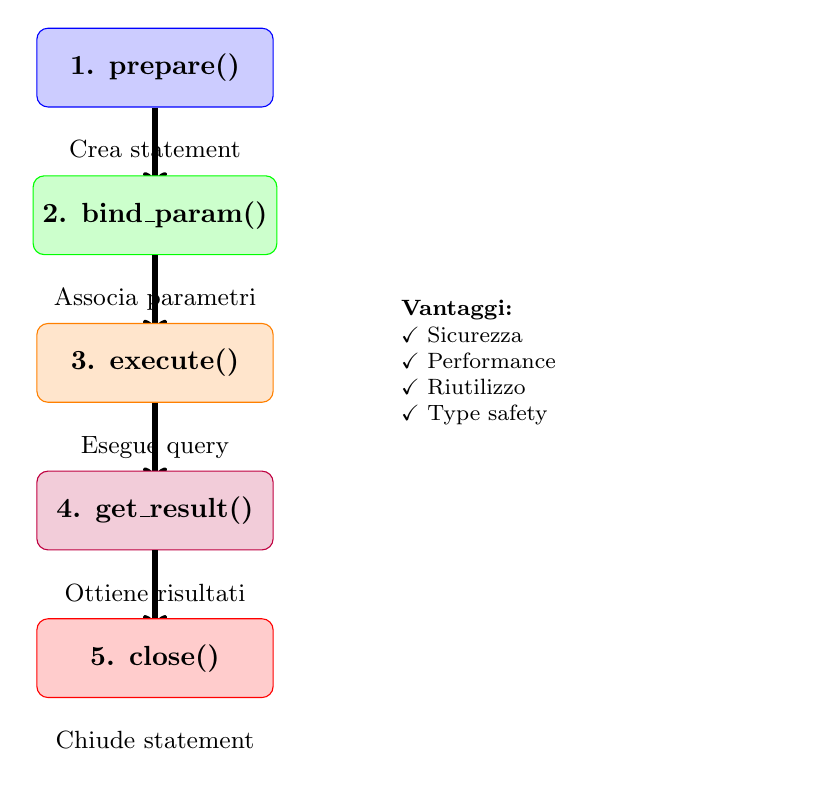
\begin{tikzpicture}[scale=0.75]
    % Passo 1
    \node[rectangle,draw=blue,fill=blue!20,minimum width=3cm,minimum height=1cm,rounded corners] (p1) at (0,5) {\textbf{1. prepare()}};
    \node[below,font=\small,text width=3cm,align=center] at (p1.south) [yshift=-0.3cm] {Crea statement};
    
    \draw[->,line width=2pt] (p1) -- (0,3);
    
    % Passo 2
    \node[rectangle,draw=green,fill=green!20,minimum width=3cm,minimum height=1cm,rounded corners] (p2) at (0,2.5) {\textbf{2. bind\_param()}};
    \node[below,font=\small,text width=3cm,align=center] at (p2.south) [yshift=-0.3cm] {Associa parametri};
    
    \draw[->,line width=2pt] (p2) -- (0,0.5);
    
    % Passo 3
    \node[rectangle,draw=orange,fill=orange!20,minimum width=3cm,minimum height=1cm,rounded corners] (p3) at (0,0) {\textbf{3. execute()}};
    \node[below,font=\small,text width=3cm,align=center] at (p3.south) [yshift=-0.3cm] {Esegue query};
    
    \draw[->,line width=2pt] (p3) -- (0,-2);
    
    % Passo 4
    \node[rectangle,draw=purple,fill=purple!20,minimum width=3cm,minimum height=1cm,rounded corners] (p4) at (0,-2.5) {\textbf{4. get\_result()}};
    \node[below,font=\small,text width=3cm,align=center] at (p4.south) [yshift=-0.3cm] {Ottiene risultati};
    
    \draw[->,line width=2pt] (p4) -- (0,-4.5);
    
    % Passo 5
    \node[rectangle,draw=red,fill=red!20,minimum width=3cm,minimum height=1cm,rounded corners] (p5) at (0,-5) {\textbf{5. close()}};
    \node[below,font=\small,text width=3cm,align=center] at (p5.south) [yshift=-0.3cm] {Chiude statement};
    
    % Annotazione laterale
    \node[right,font=\footnotesize,text width=5cm,align=left] at (4,0) {
        \textbf{Vantaggi:}\\
        $\checkmark$ Sicurezza\\
        $\checkmark$ Performance\\
        $\checkmark$ Riutilizzo\\
        $\checkmark$ Type safety
    };
\end{tikzpicture}
\end{center}
\end{frame}

% ====================
% SLIDE 58 - Riepilogo
% ====================
\begin{frame}{Riepilogo Finale}
\begin{block}{Abbiamo studiato:}
\begin{enumerate}
    \item Il DBMS MySQL e phpMyAdmin
    \item La classe MySQLi (OOP e procedurale)
    \item Connessione e gestione errori
    \item Esecuzione query e mysqli\_result
    \item Metodi fetch (assoc, row, all)
    \item Operazioni CRUD
    \item Prepared Statements per sicurezza e performance
\end{enumerate}
\end{block}

\vspace{0.3cm}
\begin{center}
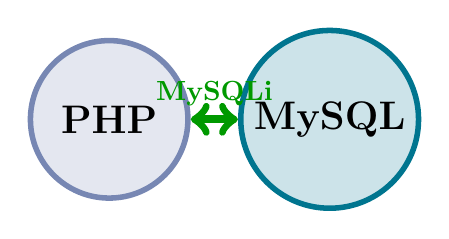
\begin{tikzpicture}[scale=0.7]
    \node[circle,draw=phpblue,fill=phpblue!20,minimum size=2cm,line width=2pt,font=\Large\bfseries] (php) at (0,0) {PHP};
    \node[circle,draw=mysqlblue,fill=mysqlblue!20,minimum size=2cm,line width=2pt,font=\Large\bfseries] (mysql) at (4,0) {MySQL};
    \draw[<->,line width=3pt,green!60!black] (php) -- node[above,font=\bfseries] {MySQLi} (mysql);
\end{tikzpicture}
\end{center}
\end{frame}

% ====================
% SLIDE 59 - Fine
% ====================
\begin{frame}
\begin{center}
{\Huge\bfseries Grazie per l'Attenzione!}

\vspace{1cm}


\begin{tikzpicture}[scale=0.8]
    % Logo PHP
    \fill[phpblue] (0,0) ellipse (1.8cm and 1.2cm);
    \node[white,font=\Huge\bfseries] at (0,0) {PHP};
    
    % Simbolo +
    \node[font=\Huge\bfseries,mysqlblue] at (3,0) {+};
    
    % Logo MySQL
    \fill[mysqlblue] (6,0) ellipse (1.8cm and 1.2cm);
    \node[white,font=\Huge\bfseries] at (6,0) {MySQL};
\end{tikzpicture}

\vspace{1cm}

\textbf{Fedeli Massimo} \\
IIS E.Fermi - Sacconi - Ceci \\
2024/25
\end{center}
\end{frame}

\end{document}
